% Options for packages loaded elsewhere
\PassOptionsToPackage{unicode}{hyperref}
\PassOptionsToPackage{hyphens}{url}
\PassOptionsToPackage{dvipsnames,svgnames,x11names}{xcolor}
%
\documentclass[
  sn-nature,
  numbered]{sn-jnl}

\usepackage{amsmath,amssymb}
\usepackage{iftex}
\ifPDFTeX
  \usepackage[T1]{fontenc}
  \usepackage[utf8]{inputenc}
  \usepackage{textcomp} % provide euro and other symbols
\else % if luatex or xetex
  \usepackage{unicode-math}
  \defaultfontfeatures{Scale=MatchLowercase}
  \defaultfontfeatures[\rmfamily]{Ligatures=TeX,Scale=1}
\fi
\usepackage{lmodern}
\ifPDFTeX\else  
    % xetex/luatex font selection
\fi
% Use upquote if available, for straight quotes in verbatim environments
\IfFileExists{upquote.sty}{\usepackage{upquote}}{}
\IfFileExists{microtype.sty}{% use microtype if available
  \usepackage[]{microtype}
  \UseMicrotypeSet[protrusion]{basicmath} % disable protrusion for tt fonts
}{}
\makeatletter
\@ifundefined{KOMAClassName}{% if non-KOMA class
  \IfFileExists{parskip.sty}{%
    \usepackage{parskip}
  }{% else
    \setlength{\parindent}{0pt}
    \setlength{\parskip}{6pt plus 2pt minus 1pt}}
}{% if KOMA class
  \KOMAoptions{parskip=half}}
\makeatother
\usepackage{xcolor}
\setlength{\emergencystretch}{3em} % prevent overfull lines
\setcounter{secnumdepth}{-\maxdimen} % remove section numbering
% Make \paragraph and \subparagraph free-standing
\ifx\paragraph\undefined\else
  \let\oldparagraph\paragraph
  \renewcommand{\paragraph}[1]{\oldparagraph{#1}\mbox{}}
\fi
\ifx\subparagraph\undefined\else
  \let\oldsubparagraph\subparagraph
  \renewcommand{\subparagraph}[1]{\oldsubparagraph{#1}\mbox{}}
\fi


\providecommand{\tightlist}{%
  \setlength{\itemsep}{0pt}\setlength{\parskip}{0pt}}\usepackage{longtable,booktabs,array}
\usepackage{calc} % for calculating minipage widths
% Correct order of tables after \paragraph or \subparagraph
\usepackage{etoolbox}
\makeatletter
\patchcmd\longtable{\par}{\if@noskipsec\mbox{}\fi\par}{}{}
\makeatother
% Allow footnotes in longtable head/foot
\IfFileExists{footnotehyper.sty}{\usepackage{footnotehyper}}{\usepackage{footnote}}
\makesavenoteenv{longtable}
\usepackage{graphicx}
\makeatletter
\def\maxwidth{\ifdim\Gin@nat@width>\linewidth\linewidth\else\Gin@nat@width\fi}
\def\maxheight{\ifdim\Gin@nat@height>\textheight\textheight\else\Gin@nat@height\fi}
\makeatother
% Scale images if necessary, so that they will not overflow the page
% margins by default, and it is still possible to overwrite the defaults
% using explicit options in \includegraphics[width, height, ...]{}
\setkeys{Gin}{width=\maxwidth,height=\maxheight,keepaspectratio}
% Set default figure placement to htbp
\makeatletter
\def\fps@figure{htbp}
\makeatother

%%%% Standard Packages

\usepackage{graphicx}%
\usepackage{multirow}%
\usepackage{amsmath,amssymb,amsfonts}%
\usepackage{amsthm}%
\usepackage{mathrsfs}%
\usepackage[title]{appendix}%
\usepackage{xcolor}%
\usepackage{textcomp}%
\usepackage{manyfoot}%
\usepackage{booktabs}%
\usepackage{algorithm}%
\usepackage{algorithmicx}%
\usepackage{algpseudocode}%
\usepackage{listings}%

%%%%

\raggedbottom
\makeatletter
\@ifpackageloaded{caption}{}{\usepackage{caption}}
\AtBeginDocument{%
\ifdefined\contentsname
  \renewcommand*\contentsname{Table of contents}
\else
  \newcommand\contentsname{Table of contents}
\fi
\ifdefined\listfigurename
  \renewcommand*\listfigurename{List of Figures}
\else
  \newcommand\listfigurename{List of Figures}
\fi
\ifdefined\listtablename
  \renewcommand*\listtablename{List of Tables}
\else
  \newcommand\listtablename{List of Tables}
\fi
\ifdefined\figurename
  \renewcommand*\figurename{Figure}
\else
  \newcommand\figurename{Figure}
\fi
\ifdefined\tablename
  \renewcommand*\tablename{Table}
\else
  \newcommand\tablename{Table}
\fi
}
\@ifpackageloaded{float}{}{\usepackage{float}}
\floatstyle{ruled}
\@ifundefined{c@chapter}{\newfloat{codelisting}{h}{lop}}{\newfloat{codelisting}{h}{lop}[chapter]}
\floatname{codelisting}{Listing}
\newcommand*\listoflistings{\listof{codelisting}{List of Listings}}
\makeatother
\makeatletter
\makeatother
\makeatletter
\@ifpackageloaded{caption}{}{\usepackage{caption}}
\@ifpackageloaded{subcaption}{}{\usepackage{subcaption}}
\makeatother
\ifLuaTeX
  \usepackage{selnolig}  % disable illegal ligatures
\fi
\usepackage[]{natbib}
\bibliographystyle{plainnat}
\usepackage{bookmark}

\IfFileExists{xurl.sty}{\usepackage{xurl}}{} % add URL line breaks if available
\urlstyle{same} % disable monospaced font for URLs
\hypersetup{
  pdftitle={Shifts in water supply and demand drive land cover change across Chile},
  pdfauthor={Francisco Zambrano; Anton Vrieling; Francisco Meza; Iongel Duran-Llacer; Francisco Fernández; Alejandro Venegas-González; Nicolas Raab; Dylan Craven},
  pdfkeywords={drought, land cover, water demand, water supply},
  colorlinks=true,
  linkcolor={blue},
  filecolor={Maroon},
  citecolor={Blue},
  urlcolor={Blue},
  pdfcreator={LaTeX via pandoc}}

\title[Shifts in water supply and demand drive land cover change across
Chile]{Shifts in water supply and demand drive land cover change across
Chile}

% author setup
\author*[1,2]{\fnm{Francisco} \sur{Zambrano}}\email{francisco.zambrano@umayor.cl}\author[3]{\fnm{Anton} \sur{Vrieling}}\author[4,5,6]{\fnm{Francisco} \sur{Meza}}\author[7]{\fnm{Iongel} \sur{Duran-Llacer}}\author[8,9]{\fnm{Francisco} \sur{Fernández}}\author[10]{\fnm{Alejandro} \sur{Venegas-González}}\author[4]{\fnm{Nicolas} \sur{Raab}}\author[11,12]{\fnm{Dylan} \sur{Craven}}
% affil setup
\affil[1]{, \orgname{Hémera Centro de Observación de la Tierra, Facultad
de Ciencias, Escuela de Ingeniería en Medio Ambiente y Sustentabilidad,
Universidad Mayor}}
\affil[2]{, \orgname{Observatorio de Sequía para la Agricultura y la
Biodiversidad de Chile (ODES), Universidad Mayor}}
\affil[3]{, \orgname{Faculty of Geo-Information Science and Earth,
University of Twente}}
\affil[4]{, \orgname{Facultad de Agronomía y Sistemas Naturales,
Pontificia Universidad Católica de Chile.}}
\affil[5]{, \orgname{Instituto para el Desarrollo Sustentable.
Pontificia Universidad Católica de Chile}}
\affil[6]{, \orgname{Centro Interdisciplinario de Cambio Global,
Pontificia Universidad Católica de Chile}}
\affil[7]{, \orgname{Hémera Centro de Observación de la Tierra, Facultad
de Ciencias, Universidad Mayor,}}
\affil[8]{, \orgname{Center of Economics for Sustainable Development
(CEDES), Faculty of Economics and Government, Universidad San
Sebastian}}
\affil[9]{, \orgname{Center of Applied Ecology and Sustainability
(CAPES)}}
\affil[10]{, \orgname{Instituto de Ciencias Agroalimentarias, Animales y
Ambientales (ICA3), Universidad de O'Higgins}}
\affil[4]{}
\affil[11]{\orgdiv{GEMA Center for Genomics, Ecology \& Environment,
Universidad Mayor, Camino La Pirámide Huechuraba 5750}}
\affil[12]{, \orgname{Data Observatory Foundation}}

% abstract 

\abstract{Globally, droughts are becoming longer, more frequent and more
severe, and their impacts are multidimensional. These impacts typically
extend beyond the water balance as long-term, cumulative changes in the
water balance can lead to regime shifts in land use. Here, we assess the
effects of temporal changes in water supply and demand on vegetation
productivity and land cover change over multiple time scales in
continental Chile, which has experienced a severe drought over the last
20 years. Across most of continental Chile, we found a persistent
decreasing trend in water supply and an increasing trend in water demand
since 1981, trends that intensify over longer time scales. This
long-term decrease in water availability has led to a decrease in
vegetation productivity, especially in central and southern Chile. Our
models suggest that increasing drought severity has led to shifts in
land use towards more drought-tolerant land cover types, such as
shrublands. We also found evidence that human perceptions of prolonged
drought can indirectly lead to large-scale changes in land use. Our
results suggest that long-term climate change may lead to regime shifts
in land cover that can be mitigated by context-specific adaptation
strategies.}

% keywords
\keywords{drought,  land cover,  water demand,  water supply}

\begin{document}
\maketitle

\section{Introduction}\label{sec-intro}

Across many regions of the world, droughts are becoming longer and more
frequent and severe \citep{Miranda2023, IPCC2023}, impacting ecosystems
via tree mortality\citep{Cheng2024} and productivity \citep{Miranda2023}
and inducing shifts in land cover and use \citep{Crausbay2017}. However,
identifying drought events is surprisingly idiosyncratic due to the
varying criteria used for classification. Droughts can be classified as
either 1) meteorological, i.e., when precipitation in a specific period
falls below mean precipitation values observed over multiple years
(usually more than 30 years); 2) hydrological, i.e., when precipitation
anomalies last for long periods (months to years) and affect water
systems; 3) agricultural, i.e.~when precipitation deficits negatively
impact plant health, leading to decreases in crop or pasture
productivity \citep{Wilhite1985}; or 4) ecological, i.e., when
precipitation deficits negatively affect the provisioning of ecosystem
services and trigger feedbacks in natural or human systems
\citep{Crausbay2017}. Such feedbacks include drought impacts on human
decision making and activities, which can lead to land-use change
\citep{VanLoon2016, AghaKouchak2021}, which may have cascading effects
on biodiversity and ecosystem services (e.g.,
\citet{Lawler2014};\citet{Newbold2015}).

Despite the high degree of confidence in the impacts of rising
temperatures on the extent, frequency, and severity of agricultural and
ecological droughts \citep{IPCC2023}, which are likely to increase even
if global warming stabilizes at 1.5°--2°C, the severity of
meteorological droughts has been remarkably stable globally over the
past century \citep{Vicente-Serrano2022, Kogan2020}. In the few regions
where drought severity has increased over this period (1900-2000),
rising temperatures have increased atmospheric evaporative demand (AED),
which has been associated with increases in agricultural land area
\citep{Vicente-Serrano2022}. Thus, rising water demand may reflect
parallel changes in land use - primarily agriculture - that can
exacerbate the effects of meteorological droughts on ecosystems.

From 1960 to 2019, land-use change has impacted approximately one-third
of the Earth's surface, which is four times more than previously
thought\citep{Winkler2021}. Despite the considerable interest in
land-use change dynamics \citep[e.g.,][]{Song2018, Winkler2021}, the
direction and magnitude of drought impacts on land cover change and
vegetation productivity remain uncertain
\citep{Chen2022, Akinyemi2021, Peng2017}. While meteorological droughts
are responsible for approximately 37\% of land cover change and
variability in vegetation productivity globally \citep{Peng2017}, there
is little support for the idea that meteorological droughts affect soil
moisture\citep{Chen2022}. However, the evidence supporting these results
is derived from only one drought index, Standardized Precipitation
Evapotranspiration Index \citep[SPEI,][]{Vicente-Serrano2010}, which
combines a proxy for water supply - precipitation - with a proxy for
water demand - AED - at one time scale (12 months). The use of only one
time scale may bias results of drought impacts towards ecosystems
dominated by plant growth forms such as grasses and herbs that respond
more rapidly to drought stress (\textless{} 12 months). This is because
physiological differences among and within dominant plant growth forms
may increase (or decrease) tolerance of drought stress
\citep{Craine2013, McDowell2022}. For example, trees growing in more
arid ecosystems typically respond over longer time scales than those in
more humid ecosystems \citep{Vicente-Serrano2014}..

Expanding analyses to include multiple dimensions of droughts can
provide complementary insights into the Earth's water balance - and its
impacts - over multiple time scales. Yet, the World Meteorological
Organization recommends the use of a single drought index for monitoring
droughts \citep{WMO2012}, i.e., the multi-scale Standardized
Precipitation Index {[}SPI; \citet{McKee1993}{]}, but is limited in that
it only looks at water supply in the form of precipitation. The SPEI
builds upon SPI by incorporating the effects of temperature on droughts,
and is now used widely for drought monitoring
\citep[e.g.,][]{Gebrechorkos2023, Liu2024}. To better disentangle the
effects of precipitation from those of temperature
\citep{Vicente-Serrano2020}, as well as to capture droughts in terms of
water demand, AED has been integrated into the Evaporative Demand
Drought Index \citep[EDDI,][]{McEvoy2016}, which is particularly
effective at detecting the rapid onset or intensification of droughts.
Indices derived from soil moisture products, such as the Soil Moisture
Deficit Index \citep[SDMI,][]{Narasimhan2005}, the Soil Moisture
Agricultural Drought Index \citep[SMADI,][]{Souza2021}, and the
Standardized Soil Moisture Index
\citep[SSI,][]{AghaKouchak2014, AghaKouchak2015} also monitor water
supply and are thought to better capture water availability for crops,
thus providing more relevant information for evaluating agricultural
droughts. In turn, ecological droughts, which capture the joint impacts
of precipitation and temperature on natural and productive ecosystems
via variation in net primary productivity
\citep{Camps-Valls2021, Paruelo2016, Helman2014}, are usually monitored
with the Normalized Difference Vegetation Index (NDVI) and derived
anomaly indices, e.g., zcNDVI \citep{Zambrano2018}. However, none of the
aforementioned drought indices directly or indirectly consider the
broader impacts of droughts on human decisions and activities -
particularly land-use change, which is critical to developing a more
holistic view of climate change impacts.

Here, we analyze the multi-dimensional impacts of drought on water
supply and demand, net primary productivity, and land-use change across
terrestrial ecosystems in continental Chile. Chile's diverse climate and
ecosystems \citep{Beck2023, Luebert2022} make it an ideal natural
laboratory for assessing the dynamic interactions between climate and
ecosystems, and potential impacts on land-use change. Additionally,
large parts of Chile have experienced severe drought conditions that
have significantly affected vegetation and water storage in recent
years; north-central Chile has faced a persistent precipitation deficit
(or ``mega-drought'') since 2010 \citep{Garreaud2017}, which has broadly
impacted native forests
\citep[e.g.,][]{Miranda2020, UrrutiaJalabert2018, Venegas2018} and
agricultural productivity
\citep[e.g.,][]{Zambrano2016, Zambrano2018, Zambrano2023}. There is also
growing evidence that this ``mega-drought'' has impacted farmers'
decision making, shifting to crop systems with shorter rotations and
lower capital costs \citep{Zuniga2021}. Given the persistent water
deficit associated with the ``mega-drought'' and its cascading effects
on the hydrological system \citep{Boisier2018}, it is critical to assess
multiple time scales that account for the cumulative impacts of this
extreme event over several years. We therefore aim to assess: i) short-
to long-term time trends in multi-scalar drought indices that capture
variation in the components of water balance, i.e., water supply and
demand; ii) temporal changes in land-use cover and vegetation
productivity, and iii) drought impacts on vegetation productivity and
land-use change across continental Chile.

Here, we analyze the multi-dimensional impacts of drought on water
supply and demand, net primary productivity, and land-use change across
terrestrial ecosystems in continental Chile. Chile's diverse climate and
ecosystems \citep{Beck2023, Luebert2022} make it an ideal natural
laboratory for assessing the dynamic interactions between climate and
ecosystems, and potential impacts on land-use change. Additionally,
large parts of Chile have experienced severe droughts conditions that
have significantly affected vegetation and water storage in recent
years; north-central Chile has faced a persistent precipitation deficit
(or ``mega-drought'') since 2010 \citep{Garreaud2017}, which has broadly
impacted native forests
\citep[e.g.,][]{Miranda2020, UrrutiaJalabert2018, Venegas2018} and
agricultural productivity
\citep[e.g.,][]{Zambrano2016, Zambrano2018, Zambrano2023}. There is also
growing evidence that this ``mega-drought'' has impacted farmers'
decision making, who now opt for crops with shorter rotations and lower
capital costs \citep{Zuniga2021}. Given the persistent water deficit
associated with the ``mega-drought'' and its cascading effects on the
hydrological system \citep{Boisier2018}, it is critical to assess
multiple time scales that account for the cumulative impacts of this
extreme event over several years. We therefore aim to assess: i) short-
to long-term time trends in multi-scalar drought indices that capture
variation in the components of water balance, i.e., water supply and
demand; ii) temporal changes in land-use cover and vegetation
productivity, and iii) drought impacts on vegetation productivity and
land-use change across continental Chile.

\section{Results}\label{results}

\subsection{Decreases in water supply and increases in water demand
strengthen over longer time
scales}\label{decreases-in-water-supply-and-increases-in-water-demand-strengthen-over-longer-time-scales}

We observed a decrease in SPI, SPEI, and SSI - proxies largely
associated with water supply - from north to south in continental Chile,
with the exception of the southernmost region (``Austral''), a trend
that became more pronounced over longer time scales
(Figure~\ref{fig-trendDIMacro}). In contrast, we found that EDDI - a
proxy for atmospheric water demand - showed a positive trend across
Chile, with a sharper increase over time scales in the north than in the
south. In general, these results suggest that declines in precipitation
have reduced water supply, while increases in temperature have increased
water demand over the past four decades.

\begin{figure}[!ht]

\centering{

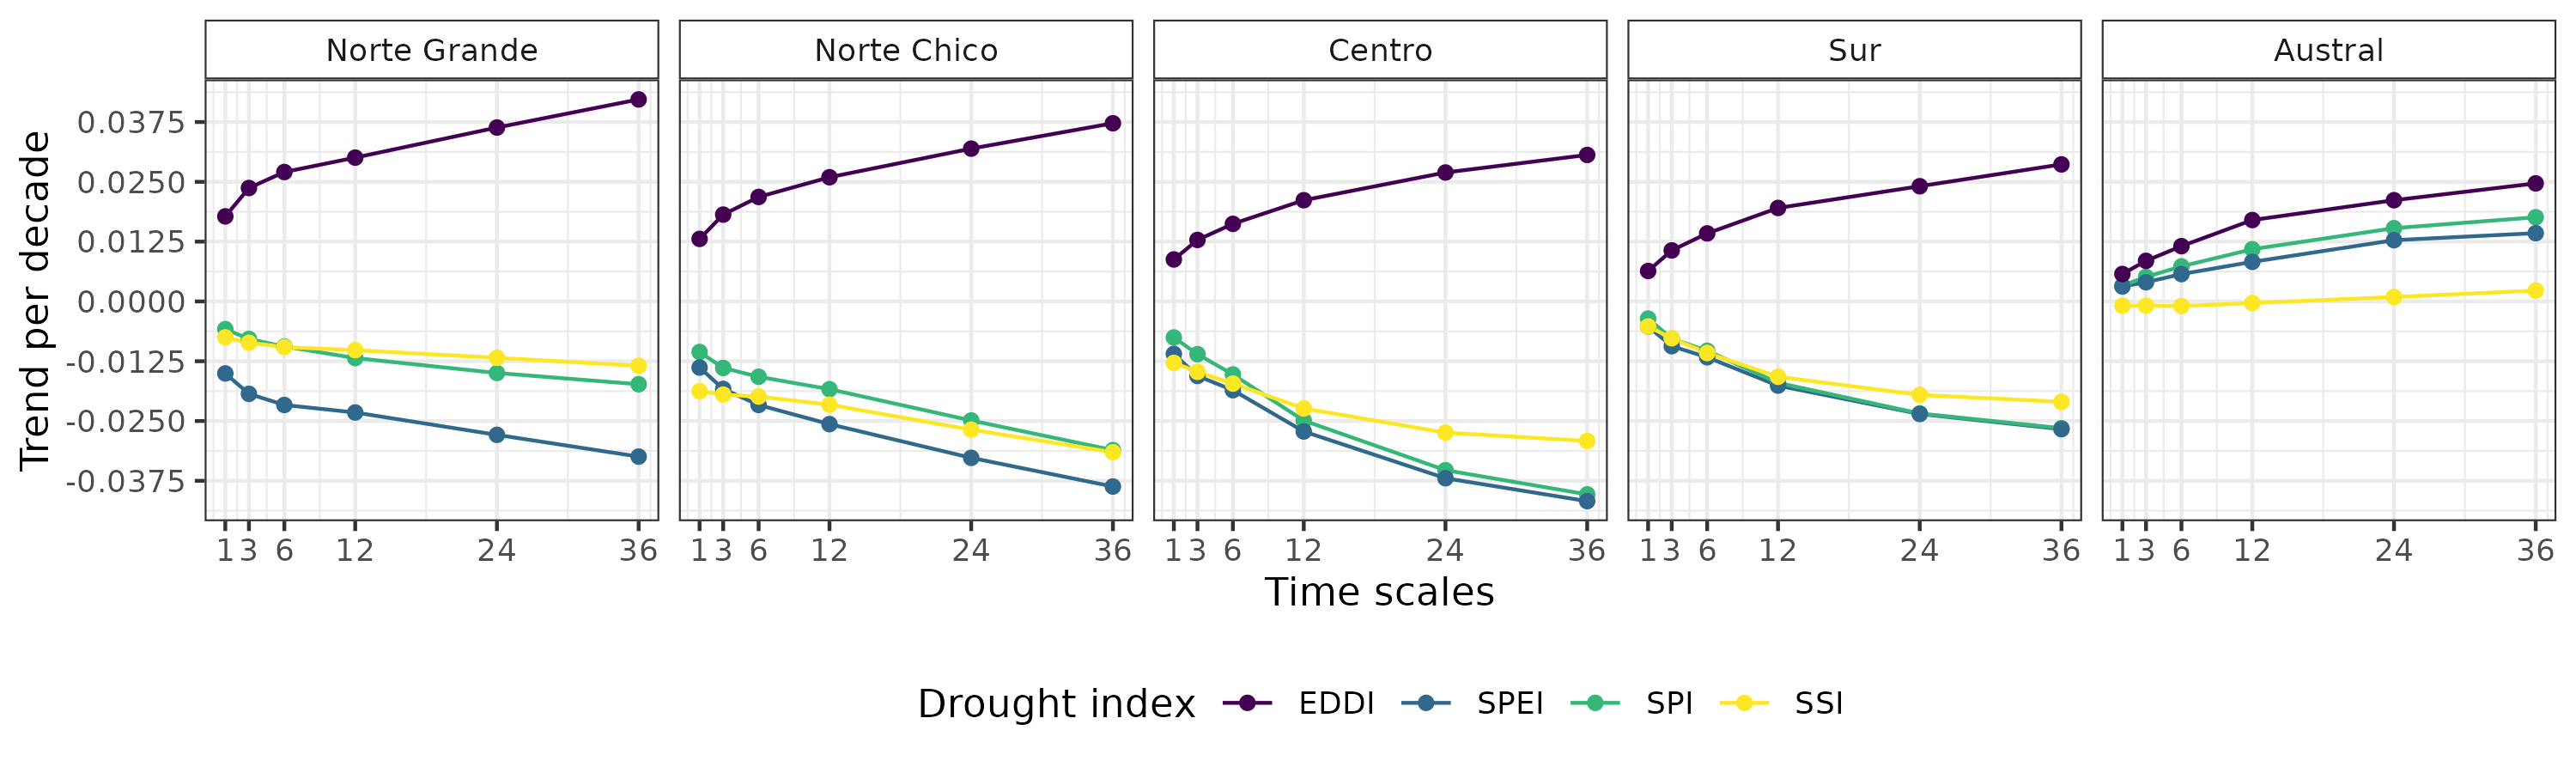
\includegraphics{figs/trend_macrozone_drought_indices.png}

}

\caption{\label{fig-trendDIMacro}\textbf{Drought severity increases over
longer time scales across most of continental Chile.} We evaluated
temporal shifts in drought severity over multiple time scales for
indices associated with water supply (SPI, SPEI, SSI) and demand (EDDI)
across continental Chile for 1981-2023. SPI is the standardized
precipitation index, SPEI is the Standardized Precipitation
Evapotranspiration Index , SSI is the Standardized Soil Moisture Index,
and EDDI is the Evaporative Demand Drought Index. Drought indices were
aggregated per region for visualization.}

\end{figure}%

\subsection{Vegetation productivity decreased in northern and central
Chile}\label{vegetation-productivity-decreased-in-northern-and-central-chile}

Despite evidence of increasing drought severity across Chile, we found
contrasting temporal trends in vegetation productivity
(Figure~\ref{fig-zcNDVI_var}). In the two southernmost regions (`Sur'
and `Austral') and one northern region (`Norte Grande'), vegetation
productivity increased over the last 23 years, while in two more central
regions (`Centro' and `Norte Chico') it decreased over the same period
(Figure~\ref{fig-zcNDVI_var}). In central Chile, vegetation productivity
was lowest from 2019 to 2022, which could be due to either a decrease in
vegetation area, a loss of biomass or browning.

\begin{figure}[!ht]

\centering{

\includegraphics{figs/temporal_variation_zcNDVI6_macrozonas_con_mapa.png}

}

\caption{\label{fig-zcNDVI_var}\textbf{Central and northern Chile have
experienced the greatest decline in vegetation productivity over the
last two decades.} Spatial (a) and temporal (b) variation in vegetation
productivity across continental Chile for 2000-2023. Vegetation
productivity was estimated as standardized vegetation productivity
(zcNDVI). Green corresponds to areas with a positive temporal trend in
zcNDVI, red corresponds to a negative temporal trend in zcNDVI, and gray
corresponds to areas that did not change over time. Temporal trends in
zcNDVI were estimated with the non-parametric modified Mann-Kendall test
for serially correlated data.}

\end{figure}%

\subsection{Cropland and forest cover shifting
southwards}\label{cropland-and-forest-cover-shifting-southwards}

During the same period, we also observed significant changes in land
cover across continental Chile (Figure~\ref{fig-temp_var_landcover}). In
northern Chile (``Norte Grande'' and ``Norte Chico''), the cover of
croplands (-12 \(km^2 yr^{-1}\)) and savannas (-70 \(km^2 yr^{-1}\))
decreased, while the cover of barren lands increased significantly (111
\(km^2 yr^{-1}\)) and the cover of forests, grasslands and shrublands
did not change (0 \(km^2 yr^{-1}\)). In central Chile (``Centro''),
croplands (-22 \(km^2 yr^{-1}\)) and savannas (-136 \(km^2 yr^{-1}\))
experienced a strong decrease in cover, but shrublands (146
\(km^2 yr^{-1}\)), grasslands (83 \(km^2 yr^{-1}\)), and barren lands
(23 \(km^2 yr^{-1}\)) increased, and forests did not change (0
\(km^2 yr^{-1}\)). In contrast, in southern Chile (``Sur''), forest
cover (397 \(km^2 yr^{-1}\)) and cropland cover (38 \(km^2 yr^{-1}\))
increased over time, with only savanna cover decreasing (-319
\(km^2 yr^{-1}\)). In the southernmost region (``Austral''), only
savanna cover increased (172 \(km^2 yr^{-1}\)), while barren land (-93
\(km^2 yr^{-1}\)) and shrubland (-37 \(km^2 yr^{-1}\)) cover decreased.
These changes in land cover suggest that agricultural cover is shifting
further south, from northern and central Chile to southern Chile, where
savannas are apparently being rapidly replaced by native and planted
forests.

\begin{figure}[!ht]

\centering{

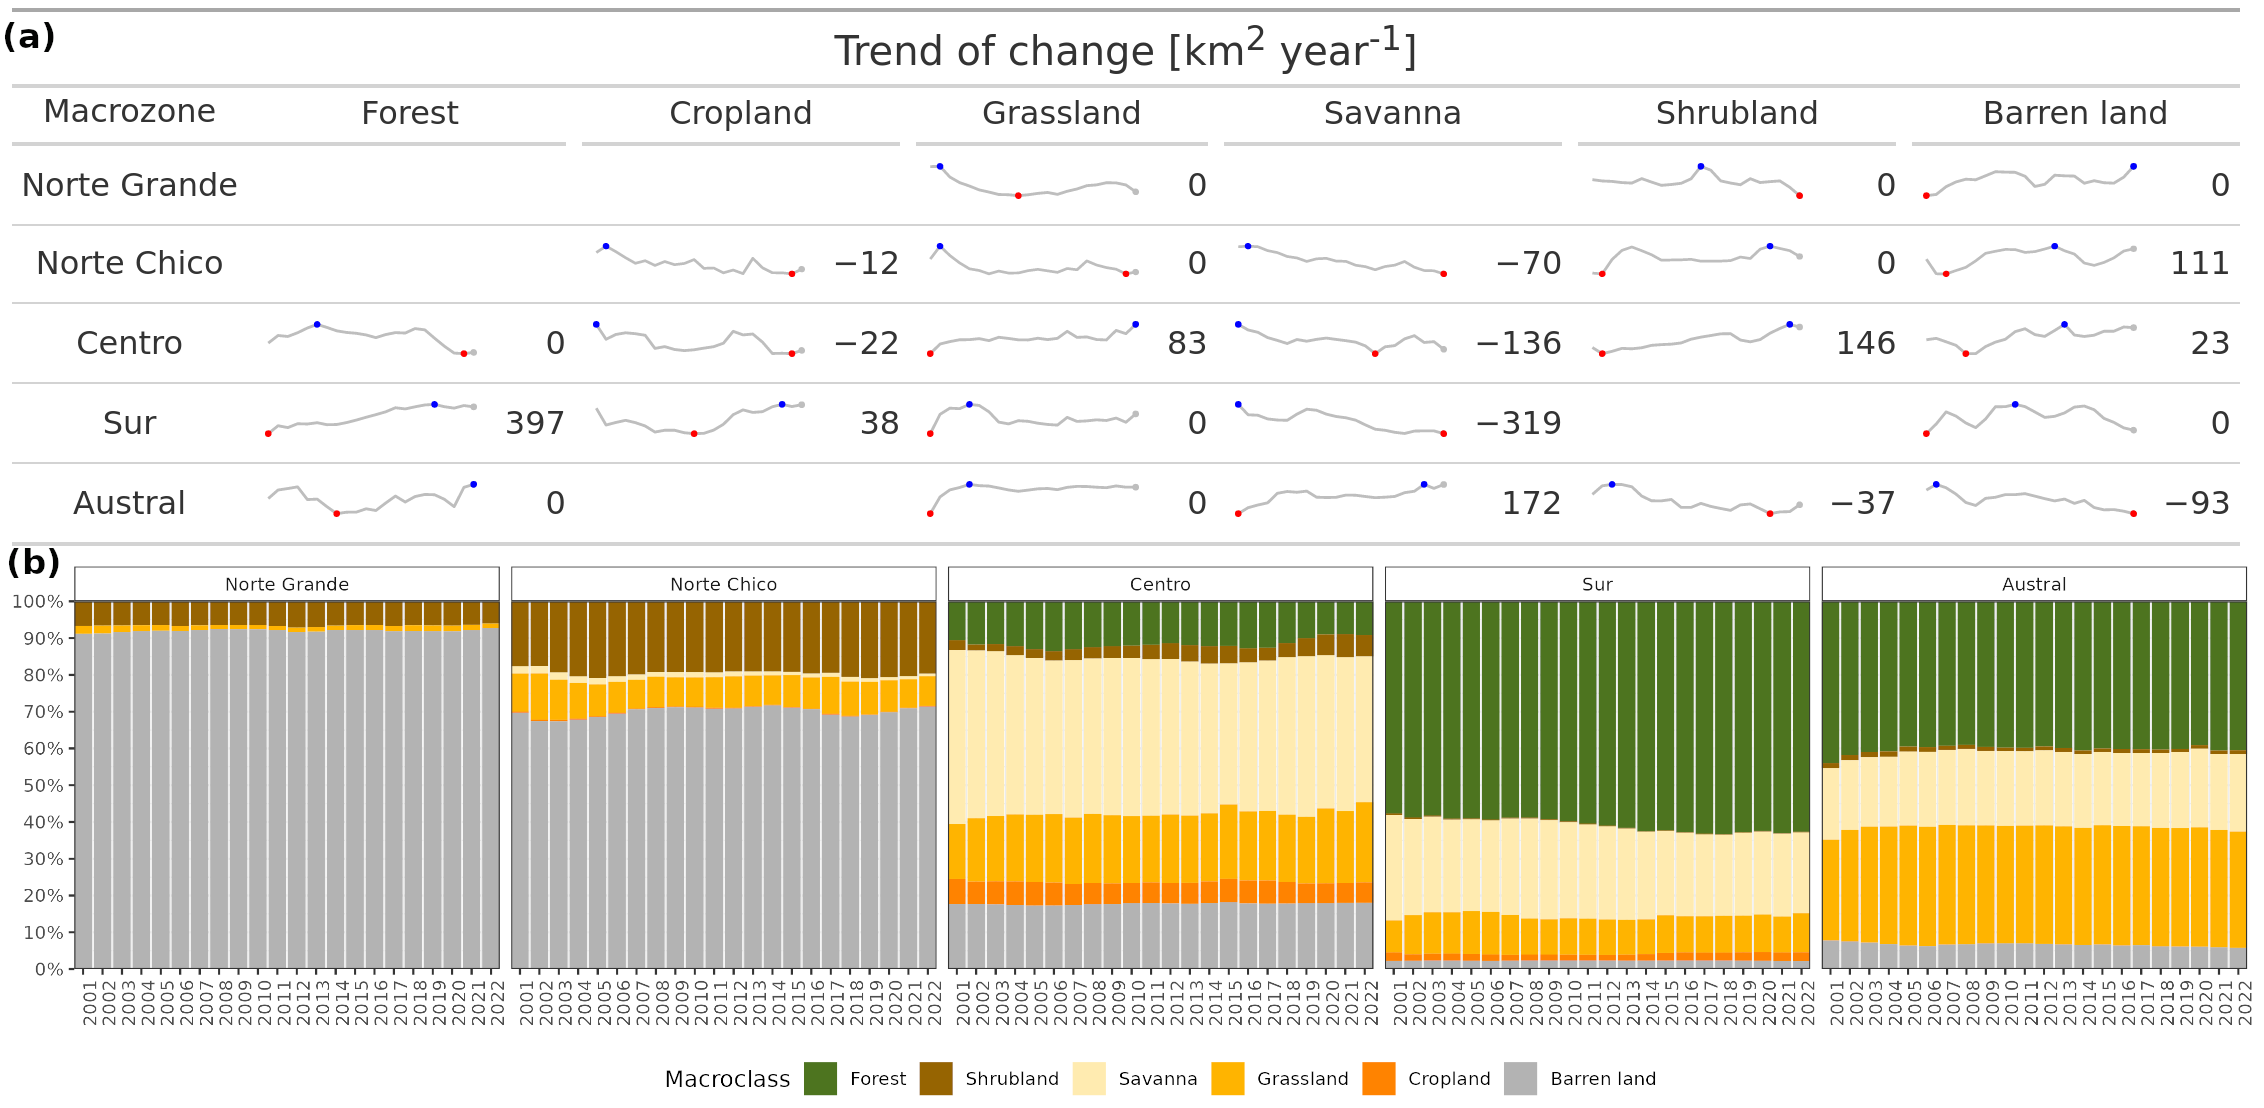
\includegraphics{figs/temporal_variation_and_trend_landcover_macroclass_2001-2022.png}

}

\caption{\label{fig-temp_var_landcover}\textbf{Land cover is shifting
dynamically across continental Chile.} Temporal trends in absolute (a)
and relative (b) land cover across continental Chile for 2001-2022.
Temporal change in land cover for each class was estimated with Sen's
slope; zero values indicate no change, while red and blue points
indicate maximum and minimum values, respectively. Land cover classes
with no values did not have statistically significant changes in area
over the study period. Relative land cover change was estimated within
each study region.}

\end{figure}%

\subsection{Vegetation productivity most strongly impacted by drought in
south-central
Chile}\label{vegetation-productivity-most-strongly-impacted-by-drought-in-south-central-chile}

We found that temporal variation in vegetation productivity was usually
best explained by drought indices with time scales greater than 12
months (Figure~\ref{fig-map_cor_r_indices}). For all drought indices,
the time scales with the strongest correlation with vegetation
productivity were longer towards northern Chile and shorter towards
southern Chile, with the exception of the southernmost region
(``Austral''). Especially in south-central Chile (``Centro'' and
``Sur''), the time scales with the strongest correlation with vegetation
productivity were concentrated in the Coastal and Andean mountain
ranges. However, the areas where vegetation was most affected by
drought, i.e.~where correlations were positive for SPI, SPEI and SSI and
negative for EDDI, were located in south-central Chile, but not
necessarily in either of the two mountain ranges. While the spatial
variation in the relationship between drought intensity and vegetation
productivity was consistent across drought indices, the drought index
that captures water supply via soil moisture (Standardized Soil Moisture
Index; SSI) tended to show a stronger correlation with vegetation
productivity over larger areas than the other drought indices.

Our analysis also revealed that water demand and supply differentially
affected the time scales at which vegetation productivity of land cover
types within each region was most impacted by drought
(Figure~\ref{fig-map_selec_time_scales_indices} /Table SSX). In northern
Chile, all land cover types exhibited stronger correlations with drought
indices associated with water supply, i.e.~SPI, SPEI, and SSI, at
shorter time scales (12 or 14 months) than those associated with water
demand, AED (36 months). In central Chile, we observed a similar pattern
for shrublands and savannas, and found that vegetation productivity of
shrublands, savannas, and croplands were generally more affected by
changes in water supply than grasslands, croplands, or forests. In
southern Chile, vegetation productivity within land cover types was less
affected by variation in water supply or demand - and at shorter
timescales than in other regions. Notably, vegetation productivity of
native and planted forests was weakly correlated with drought indices (r
\textless{} 0.2) at relatively long time scales, particularly in central
Chile.

\begin{figure}[!ht]

\centering{

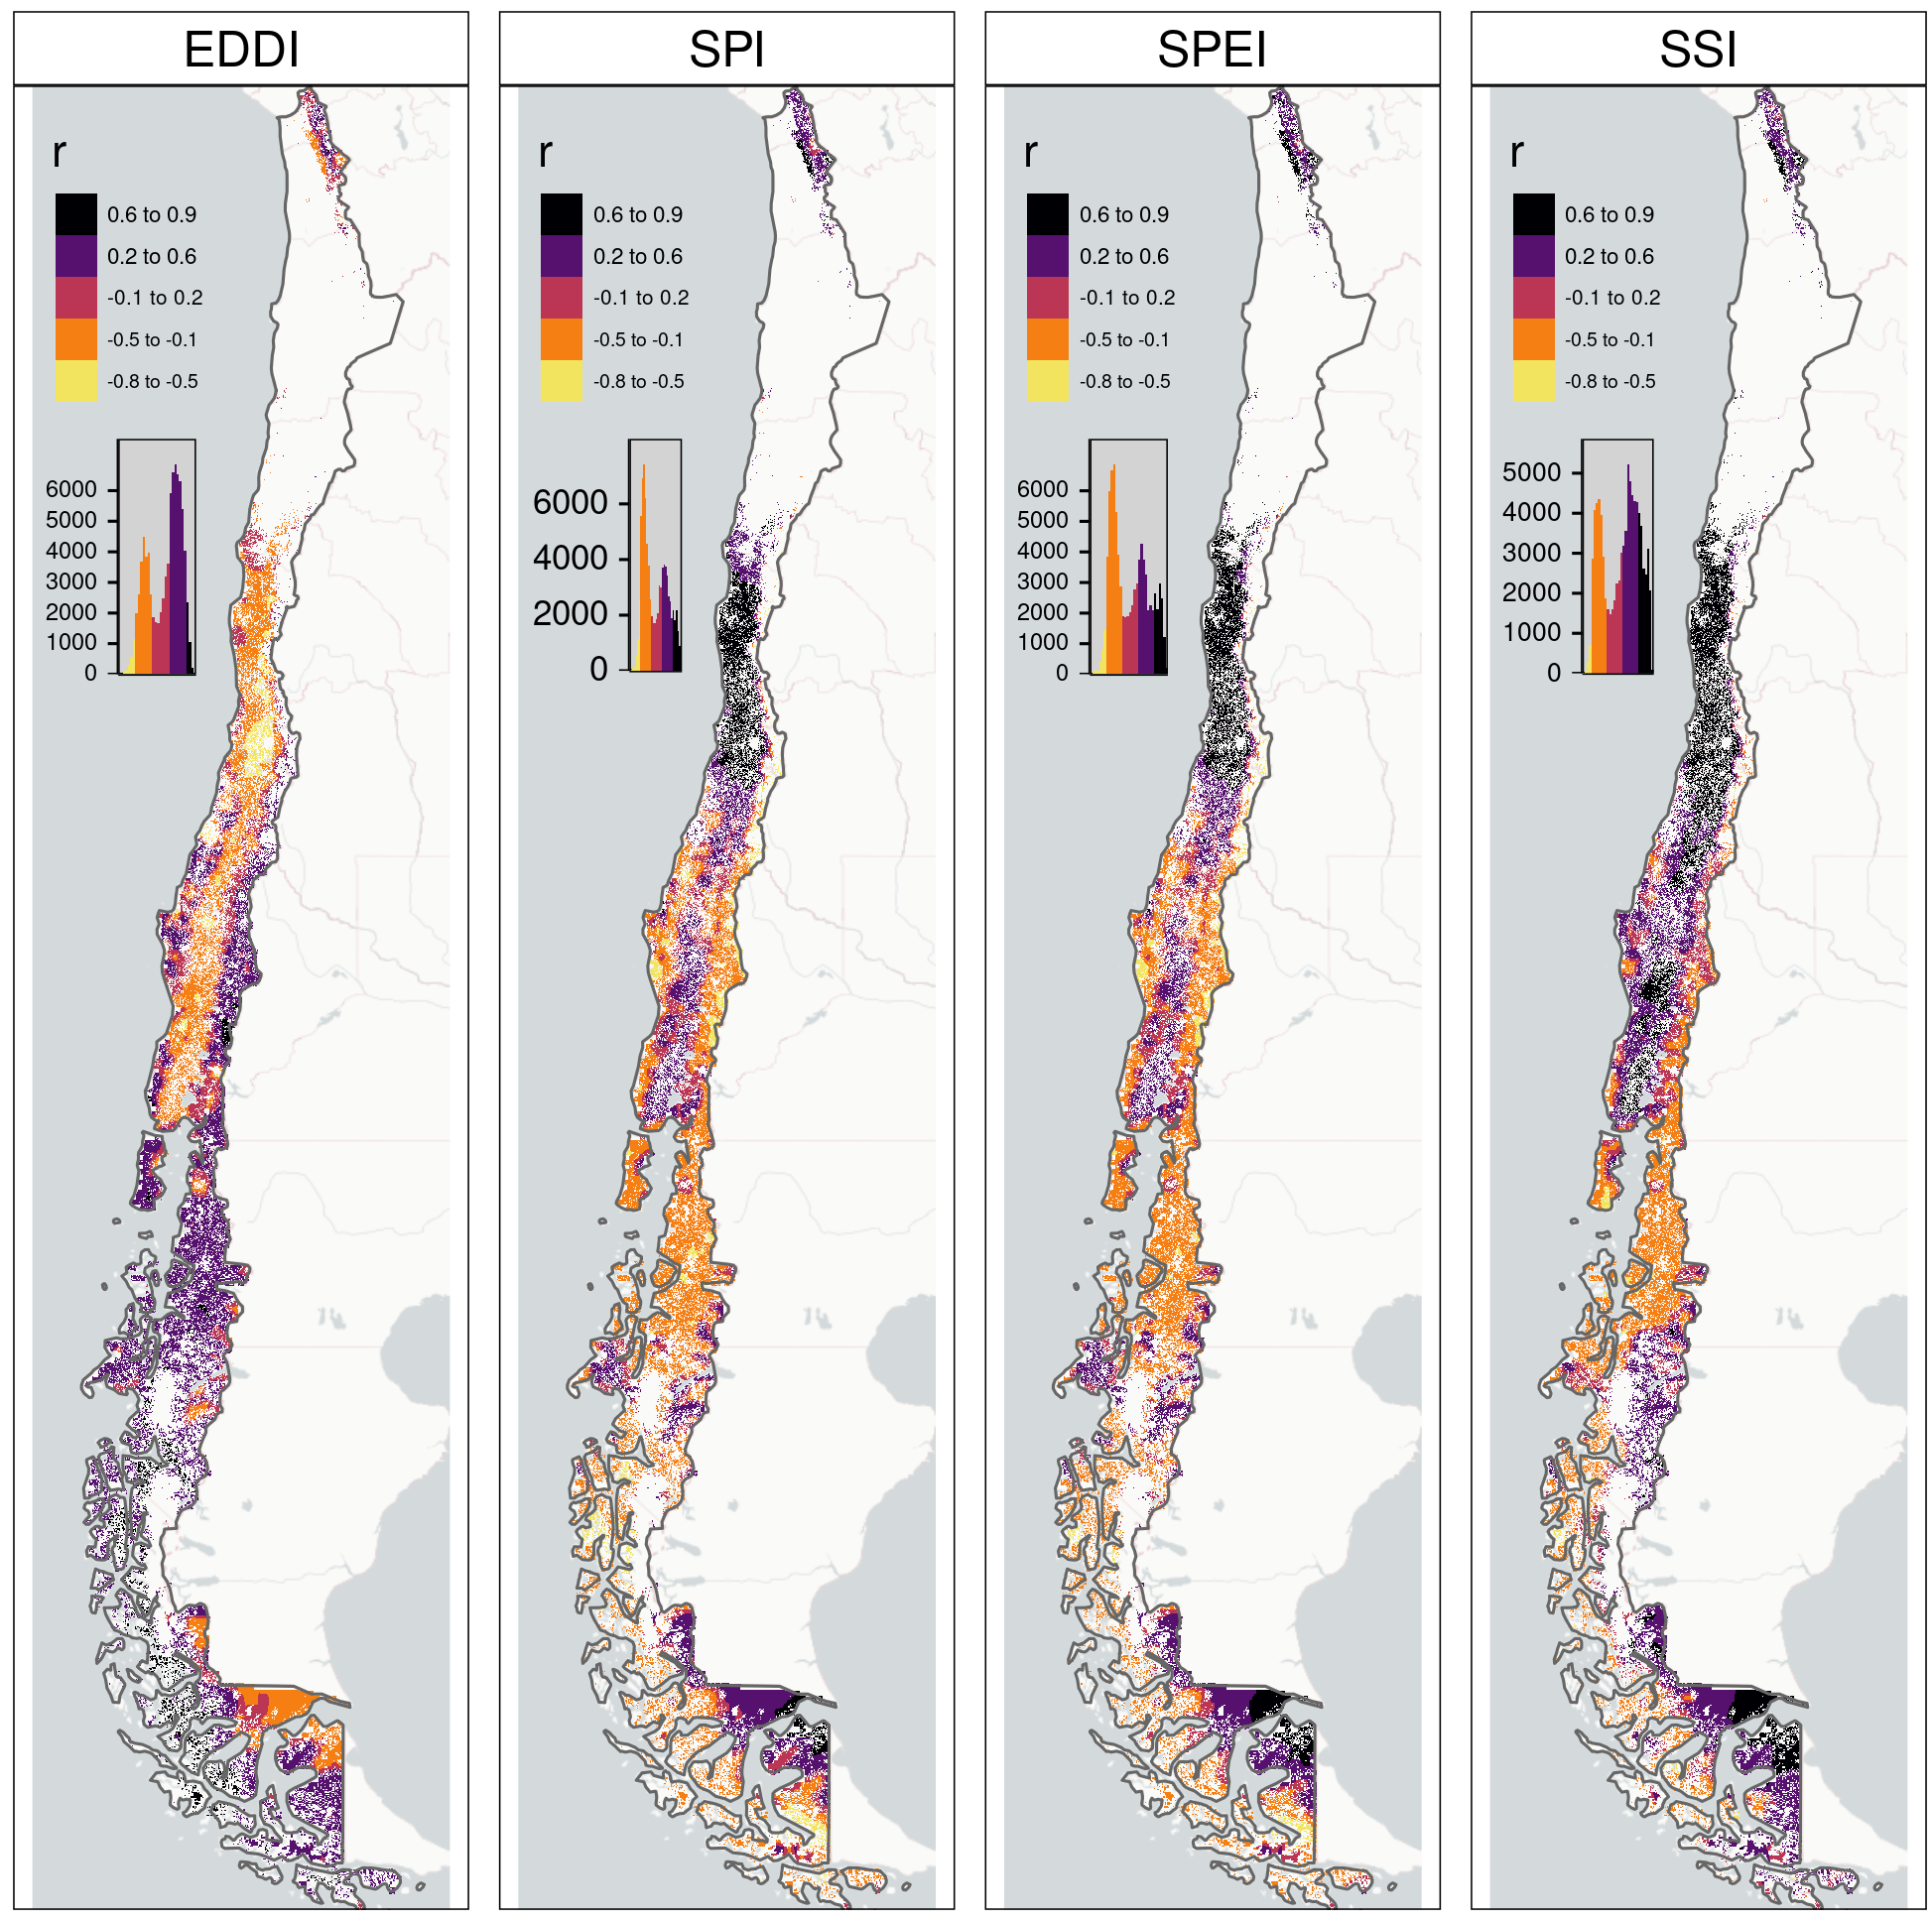
\includegraphics{figs/mapa_cor_r_indices_zcNDVI6.png}

}

\caption{\label{fig-map_cor_r_indices}\textbf{Drought impacts on
vegetation productivity shift from north to south across continental
Chile.} Pearson's correlation coefficient was used to estimate the
direction and magnitude of the relationship between drought severity and
vegetation productivity for each index. We show Pearson correlation
coefficients for the time scale (3 - 36 months) at which they reach
their maximum value. Areas in white indicate no statistically
significant correlation.}

\end{figure}%

\begin{figure}[!ht]

\centering{

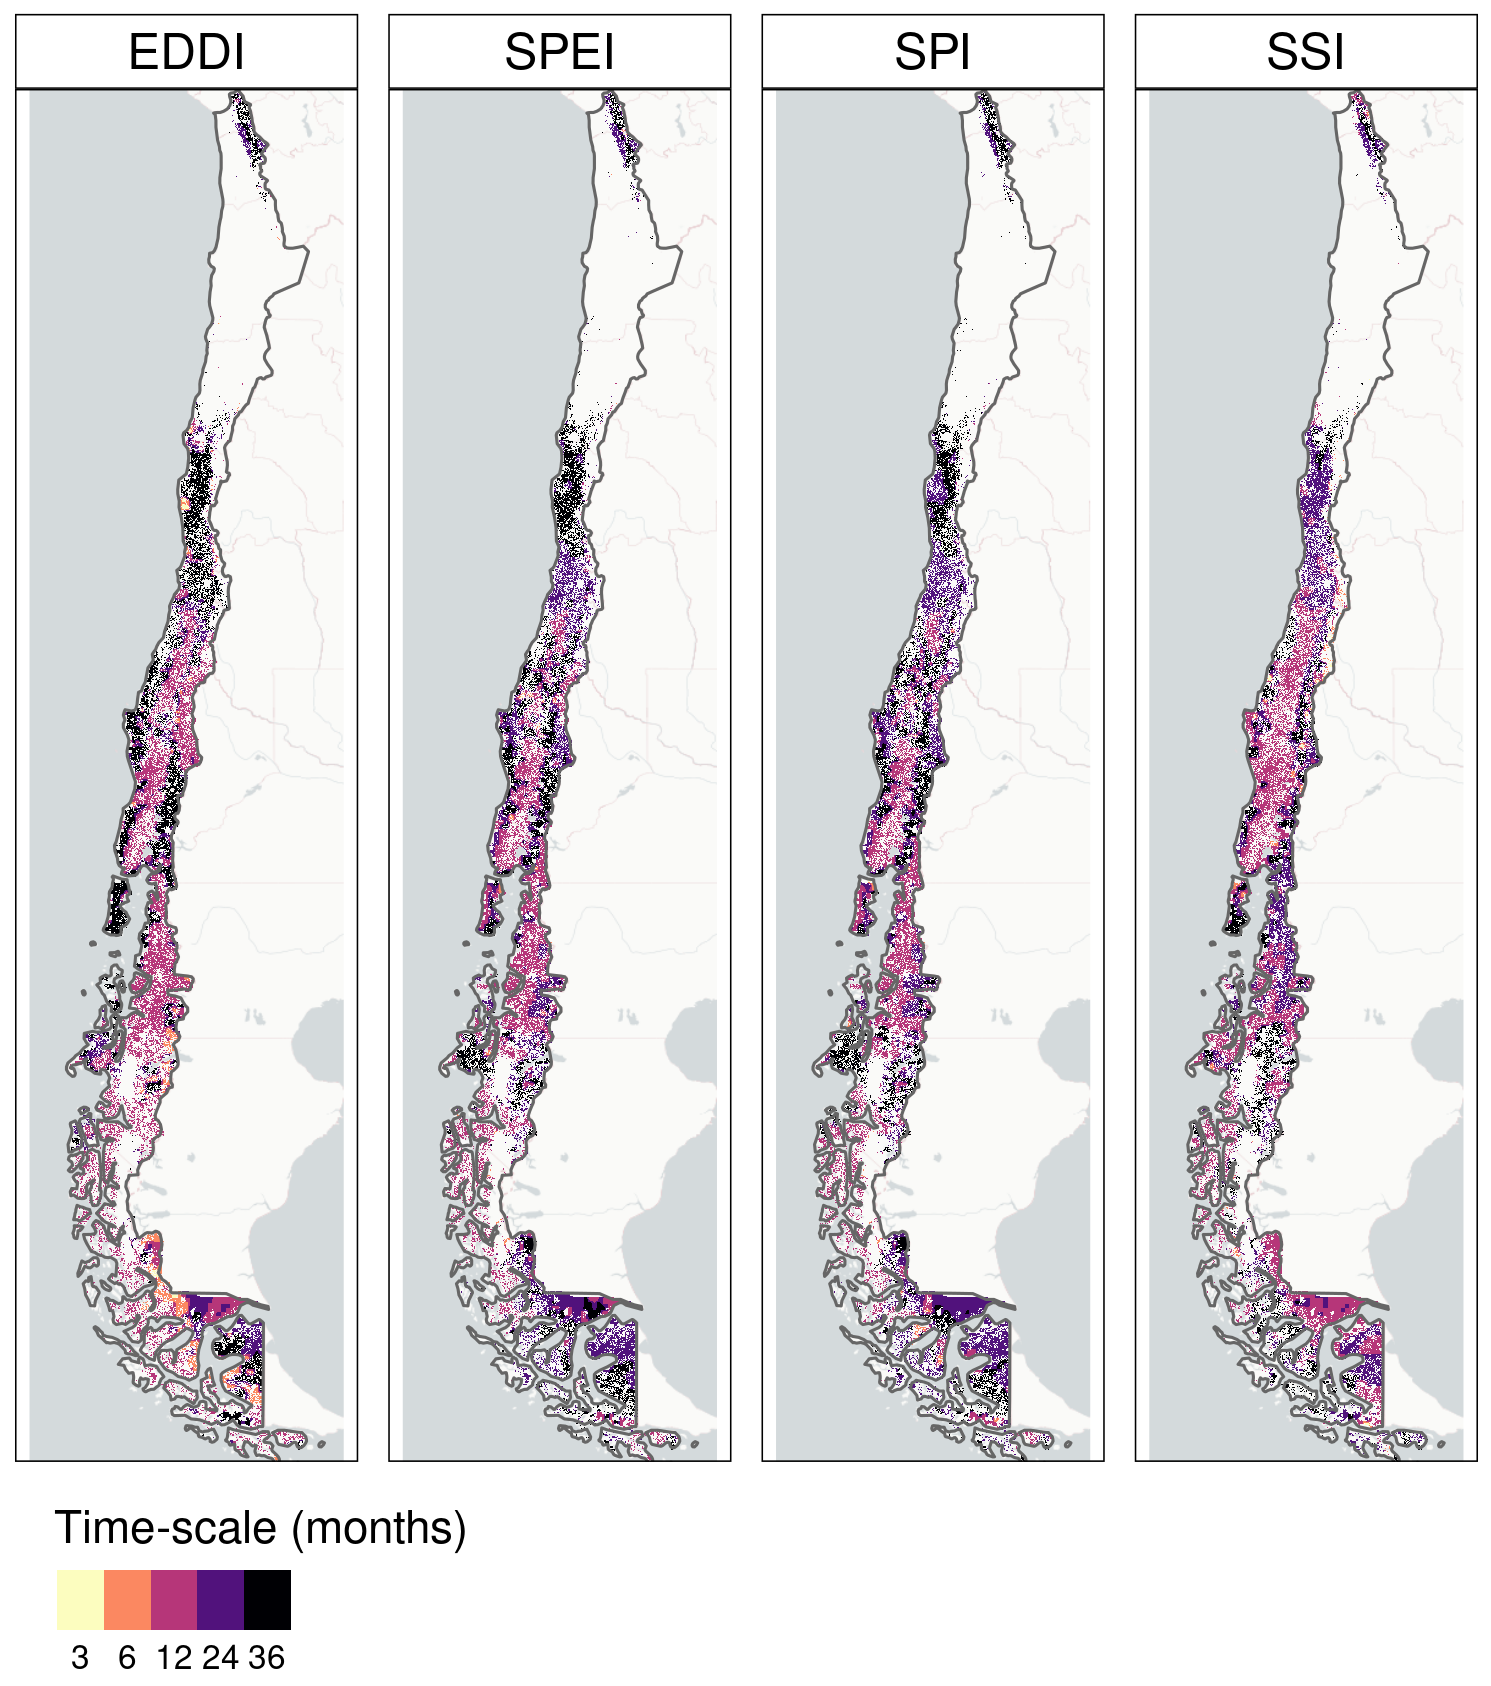
\includegraphics{figs/mapa_cor_selec_indices_zcNDVI6.png}

}

\caption{\label{fig-map_selec_time_scales_indices}\textbf{Drought
impacts on vegetation productivity are higher over longer time scales
across continental Chile.} Spatial variation in the time scale (3-36
months) at which drought impacts on vegetation productivity are most
severe across continental Chile. White spaces indicate no significant
correlation between vegetation productivity and drought severity.}

\end{figure}%

\subsection{Drought transforms land cover
distribution}\label{drought-transforms-land-cover-distribution}

Our random forest models show that drought indices explain between
22-48\% of the variation in land cover change across continental Chile,
with the exception of croplands whose variation was weakly affected by
drought (Figure~\ref{fig-rel_import_RF}; 11-20\%). Moreover, these
results highlight the importance of considering water supply and demand,
as drought indices associated with both aspects of water balance had
high importance values across most study regions and land cover types.
The variation in the time scale of drought indices within study regions
also suggests that different types of vegetation are not equally
sensitive to droughts of similar intensities. For example, changes in
savanna and shrubland cover were associated with longer time scales in
most regions, while changes in forest cover in central and southern
Chile were associated with shorter time scales. Our results also show
that drought severity was associated with the magnitude and direction of
land cover change (Figure~\ref{fig-parcial_variation}). More
specifically, we found that decreases in precipitation (SPI-6) and soil
moisture (SSI-36) and increases in atmospheric evaporative demand
(EDDI-6 and EDDI-36) at multiple time scales are associated with
non-linear decreases in grassland across continental Chile and forest
cover from central to southern Chile. In contrast, shrubland increased
non-linearly in response to decreases in precipitation (SPI-6 and
SPI-36) and soil moisture (SSI-6 and SSI--36) and increases in
atmospheric evaporative demand (EDDI-6 and EDDI-36) across central and
northern Chile. Savanna cover responded weakly to changes in
precipitation across continental Chile, but exhibited more pronounced
non-linear declines in response to increasing atmospheric evaporative
demand (EDDI-6 and EDDI-36) across most study regions. Cropland cover,
not surprisingly, varied weakly in response to changes in either water
supply or demand.

\begin{figure}[!ht]

\centering{

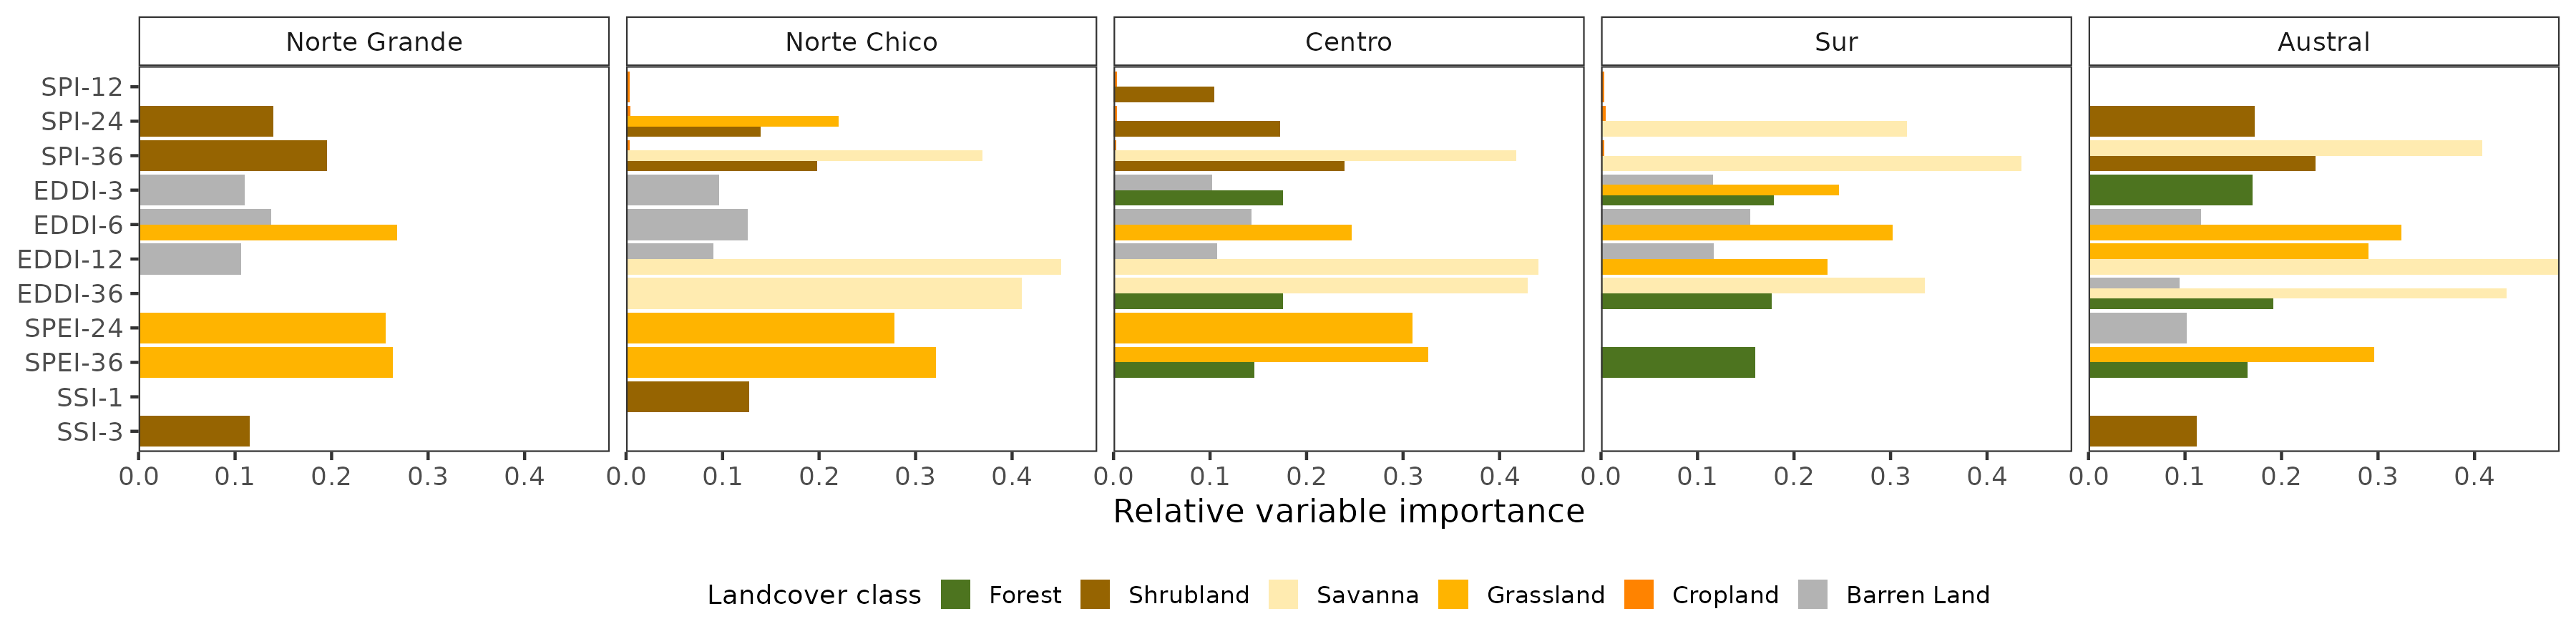
\includegraphics{figs/bars_relative_importance_RF.png}

}

\caption{\label{fig-rel_import_RF}\textbf{Shifts in water supply and
demand drive land cover change across multiple time scales.} Variable
importance of multi-scalar drought indices for explaining land cover
change in five study regions across continental Chile. Variable
importance was estimated with Random Forest models fitted for each
combination of study region and land cover type. SPI is the Standardized
Precipitation index, SPEI is the Standardized Precipitation
Evapotranspiration Index , SSI is the Standardized Soil Moisture Index,
and EDDI is the Evaporative Demand Drought Index. The numbers next to
the drought index correspond to the time scales in months (1- 36)}

\end{figure}%

\begin{figure}[!ht]

\centering{

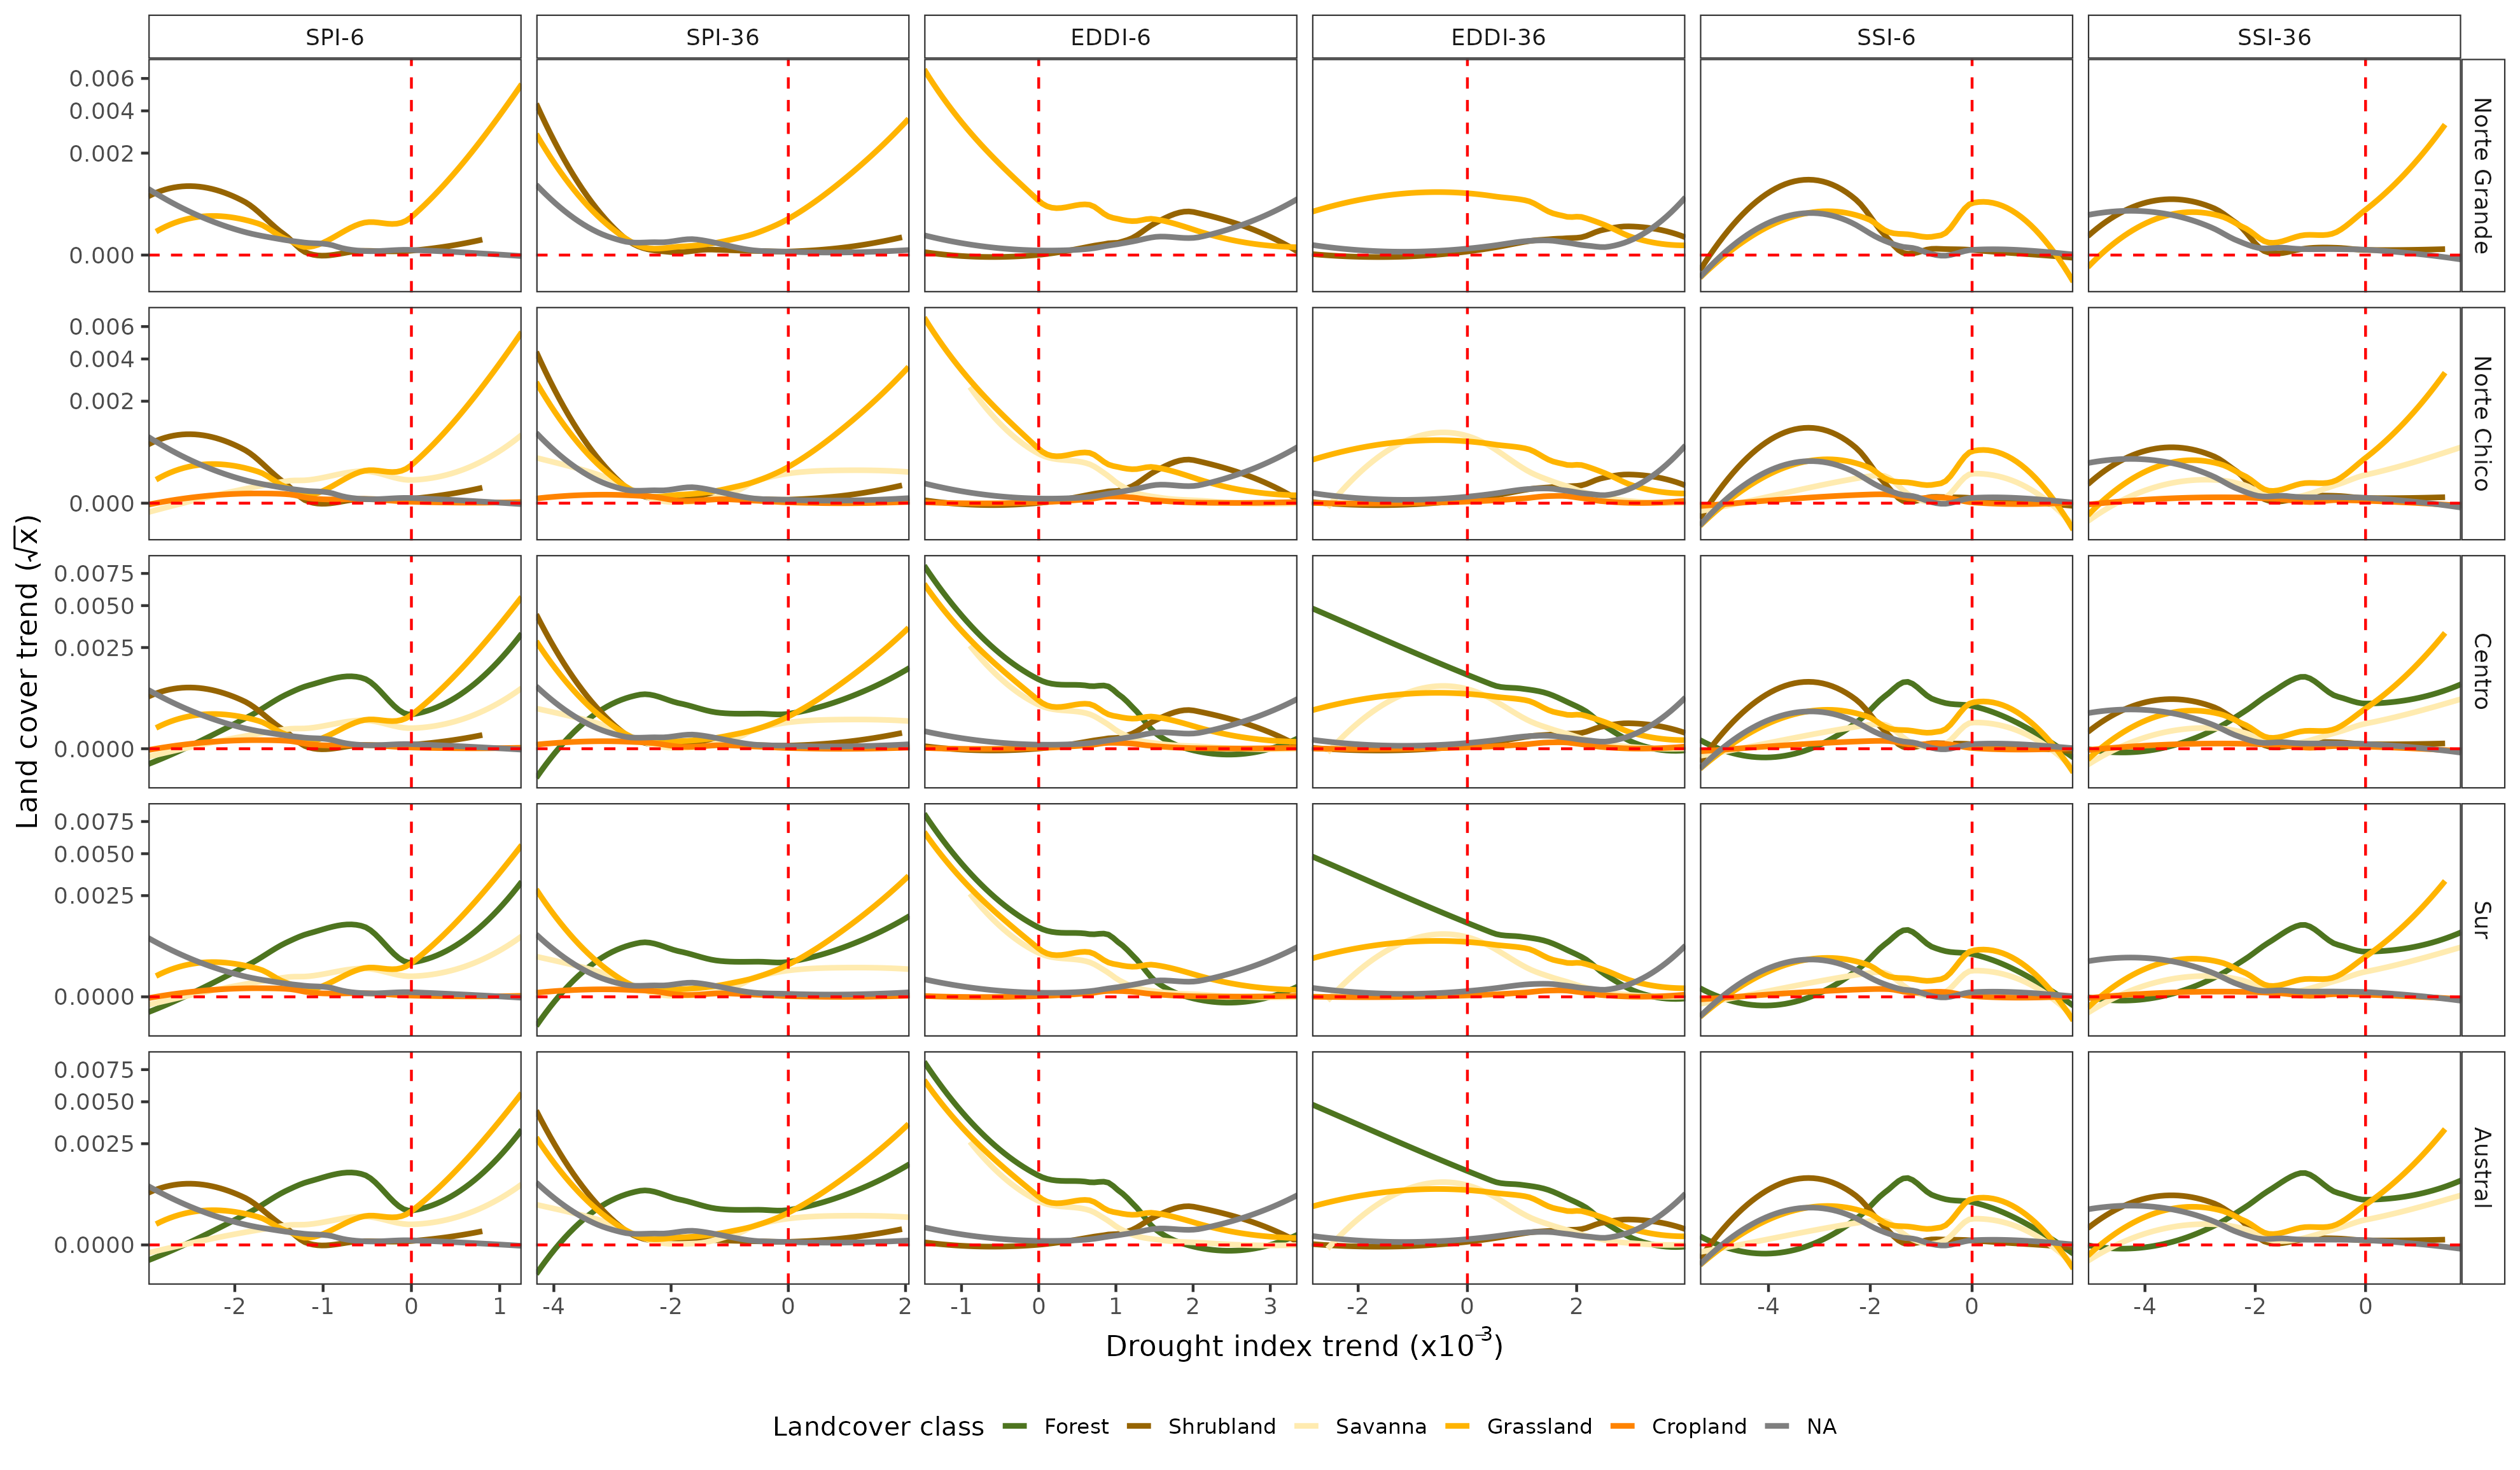
\includegraphics{figs/RF_most_important_variables_trend_LC_vs_trend_DI.png}

}

\caption{\label{fig-parcial_variation}\textbf{Drought severity drives
land cover change, but not for all cover types.} Response of land cover
change in response to water demand and supply across multiple time
scales and study regions in continental Chile. SPI is the standardized
precipitation index, SPEI is the Standardized Precipitation
Evapotranspiration Index, SSI is the Standardized Soil Moisture Index,
and EDDI is the Evaporative Demand Drought Index. Numbers next to the
drought index correspond to the time scales in months (1- 36). Fitted
lines are smoothed response curves across river basins in each region
estimated with Random Forest models.}

\end{figure}%

\section{Discussion}\label{discussion}

\subsection{Temporal trends in water supply and
demand}\label{temporal-trends-in-water-supply-and-demand}

With the exception of the southernmost region, we found a significant
decreasing trend in water supply (SPI, SPEI, and SSI) over the past four
decades across continental Chile and is strongest in northern and
central Chile \citep{Boisier2018, Sarricolea2019}. Our results reveal
that decreases in water supply increased over longer time scales, which
is consistent with a progressive intensification of drought severity
across much of Chile, as has been observed in other regions experiencing
long-term droughts\citep{Rashid2019, Miro2023}. In parallel, we observed
an increased water demand (EDDI) due to rising air temperatures, which
also strengthened over longer time scales. Taken together, our results
provide multiple lines of evidence that continental Chile has
experienced a sustained drying trend due to a concurrent decrease in
precipitation and increase in atmospheric evaporative demand
\citep{Pascoa2021}.

With the exception of the southernmost region, we found a significant
decreasing trend in water supply (SPI, SPEI, and SSI) over the past four
decades across continental Chile and is strongest in northern and
central Chile \citep{Boisier2018, Sarricolea2019}. Our results reveal
that decreases in water supply increased over longer time scales, which
is consistent with a progressive intensification of drought severity
across much of Chile, as has been observed in other regions experiencing
long-term droughts \citep{Rashid2019, Miro2023}. In parallel, we
observed an increased water demand (EDDI) due to rising air
temperatures, which also strengthened over longer time scales. Taken
together, our results provide multiple lines of evidence that
continental Chile has experienced a sustained drying trend due to a
concurrent decrease in precipitation and increase in atmospheric
evaporative demand \citep{Pascoa2021}.

\subsection{Temporal trends in vegetation
productivity}\label{temporal-trends-in-vegetation-productivity}

The consequences of the persistent drying trend for ecosystems
throughout continental Chile are manifold. First, the prolonged
hydrological drought, i.e.~precipitation deficit, has reduced
groundwater storage \citep[SSI,][]{Taucare2024}, leading to a steady
decline in vegetation productivity (zcNDVI) since 2000 across northern
and central Chile, reaching its lowest level between 2020 and 2022. This
decline was most strongly associated with declines in soil moisture, as
has been reported for natural and productive ecosystems
\citep{Nicolai-Shaw2017, Jiang2020, Zhou2021}. Second, the strong
coupling between vegetation productivity and soil moisture over longer
time scales \citep{Bonan2008} that we observed provides a more direct
physiological explanation for the sharp decline in forest growth and
productivity in central Chile \citep[e.g.,][]{Miranda2023, Venegas2022},
as the dominant woody vegetation (e.g., trees, shrubs) in this region is
likely to obtain water from deeper in the soil profile than herbs,
grasses, or agricultural crops\citep{Oliviera2005}. Moreover, the
strengthening of the correlation between vegetation productivity and
water supply (SPI, SPEI, SSI) or demand (EDDI) over multiple time scales
(up to 36 months) and across land cover types
(Figure~\ref{fig-map_selec_time_scales_indices}) - demonstrates the
impacts of climate change on the water balance in Chile. Impacts may
extend beyond vegetation productivity, as reduced soil moisture in
central Chile and the western United States has increased wildfire
activity \citep{Holden2018, Gonzalez2018}, which is a growing concern in
Chile and may be further exacerbated by extensive plantations of highly
flammable tree species, e.g., Eucalyptus spp. and Pinus
spp.\citep{Bowman2019}. Third, we found that the decline in the
vegetation productivity of croplands is due to a decrease in the water
supply to a greater extent than to an increase in water demand
\citep{Quiring2010}, despite evidence that more water-intensive crops
have replaced less water-intensive crops in central Chile, leading to an
increase in water extraction from rivers or groundwater
\citep{Munoz2020, Duran2020}.

\subsection{Drought impacts on land
cover}\label{drought-impacts-on-land-cover}

We found evidence that temporal decreases in water supply and decreases
in water demand are driving shifts not only in vegetation productivity
but also in land cover across most of continental Chile. Forest and
grassland cover were particularly sensitive to changes in the water
balance over short and long temporal scales, which is consistent with
recent studies showing that progressive, long-term water deficits in
central Chile have triggered forest browning and declines in native
forest productivity \citep{Miranda2020, Venegas2022, Miranda2023}. While
our analysis do not distinguish between native and planted forests, the
latter of which are considered to be more drought tolerant in central
and southern Chile \citep{Carrasco2022}, we show that forest area
declines more sharply in response to increasing water demand due to
rising temperatures (EDDI) than decreasing water supply \citep[e.g.,
SPI, SSI,][]{Fajardo2019, Holz2018}, which may have cascading impacts on
multiple facets of forest diversity \citep{Segovia2021, Sabatini2022}.
Our results extend the results of these studies by showing that
drought-induced forest cover decline has extended beyond central Chile
to the southernmost region of continental Chile. This is noteworthy
because declines in vegetation productivity in southern Chile - a region
whose water balance is typically projected to be less affected by
climate change than central and northern Chile \citep{Breda2020} - have
only manifested since 2022 (Figure~\ref{fig-zcNDVI_var}). Moreover, our
results provide evidence that, in addition to forest cover, other land
cover types have been affected by water deficits, particularly
grasslands, despite physiological differences between dominant plant
growth forms \citep[e.g., trees, shrubs, C3 and C4
grasses,][]{Craine2013, McDowell2022}. Our results therefore suggest
that multiple land cover types could be vulnerable to regime shifts
towards more drought tolerant land cover types
\citep{Scheffer2001, Martinez-Vilalta2016}, such as shrublands, whose
cover increased non-linearly in response to increasing drought severity.
In central Chile, for example, the increase in shrubland cover could be
due to drought-induced decreases in savanna or cropland cover. Changes
in cropland cover may not be a direct consequence of drought
(Figure~\ref{fig-parcial_variation}), but rather an indirect one,
possibly reflecting the decision of resource-poor farmers to migrate to
regions with more abundant water resources or to change economic
activity \citep{AghaKouchak2021, Hermans2021}. In contrast, the increase
in shrubland cover due to a decrease in savanna cover may be ecological,
as shrubs may be more drought tolerant than other growth forms
\citep{Eldridge2011, Gotmark2016}.

Overall, our results show that long-term declines in water supply and
demand have induced widespread, multi-dimensional impacts on the
vegetation productivity and on the extent of land cover types. While
prolonged droughts may directly cause shifts to more drought-tolerant
land cover types, such as shrublands, they may also influence land cover
change through human decision making and activities. This study extends
current understanding of drought impacts by demonstrating how their
multidimensionality emerges over multiple time scales and across land
cover types, which can contribute to developing context-specific
adaptation strategies for agriculture, biodiversity conservation, and
natural resource management.

\section{Materials and Methods}\label{materials-and-methods}

\subsection{Study area}\label{study-area}

Continental Chile has a diverse climate, with strong gradients from
north to south and east to west \citep{Aceituno2021}
(Figure~\ref{fig-studyArea} a), which, together with its complex
topography, determine its ecosystem diversity
\citep{Garreaud2009, Luebert2022} (Figure~\ref{fig-studyArea} c). We
divided Chile into five regions: ``Norte Grande'' (17°34'--25°42'S),
``Norte Chico'' (25°42'-32°8'S), ``Centro'' (32°08'-36°12'S), ``Sur''
(36°12'-43°48'S), and ``Austral'' (43°48'-56°00'S). ``Norte Grande'' and
``Norte Chico'' are predominantly arid with hot (Bwh in the
Koppen-Geiger classification) and cold (Bwk) temperatures. Towards the
south of ``Norte Chico'', the climate changes to an arid steppe with
cold temperatures (Bsk). In these two northern regions, the land is
mostly bare, with a small area covered by shrublands and grasslands. In
the ``Centro'' region and the northern half of ``Sur'', the climate is
mostly Mediterranean, with warm to hot summers (Csa and Csb). Land cover
in the ``Centro'' region consists of a significant amount of shrublands
and savannas (50\%), followed by grasslands (16\%), forests (8\%), and
croplands (5\%). The south of ``Sur'' and the north of the ``Austral''
region have a mostly oceanic climate (Cfb). Those zones have a large
area of forests and grasslands. The southern part of the country has a
tundra climate, while ``Austral'' is a cold, semi-arid area covered by
grasslands and forests, and, to a lesser extent, savannas.

\begin{figure*}[!ht]

\centering{

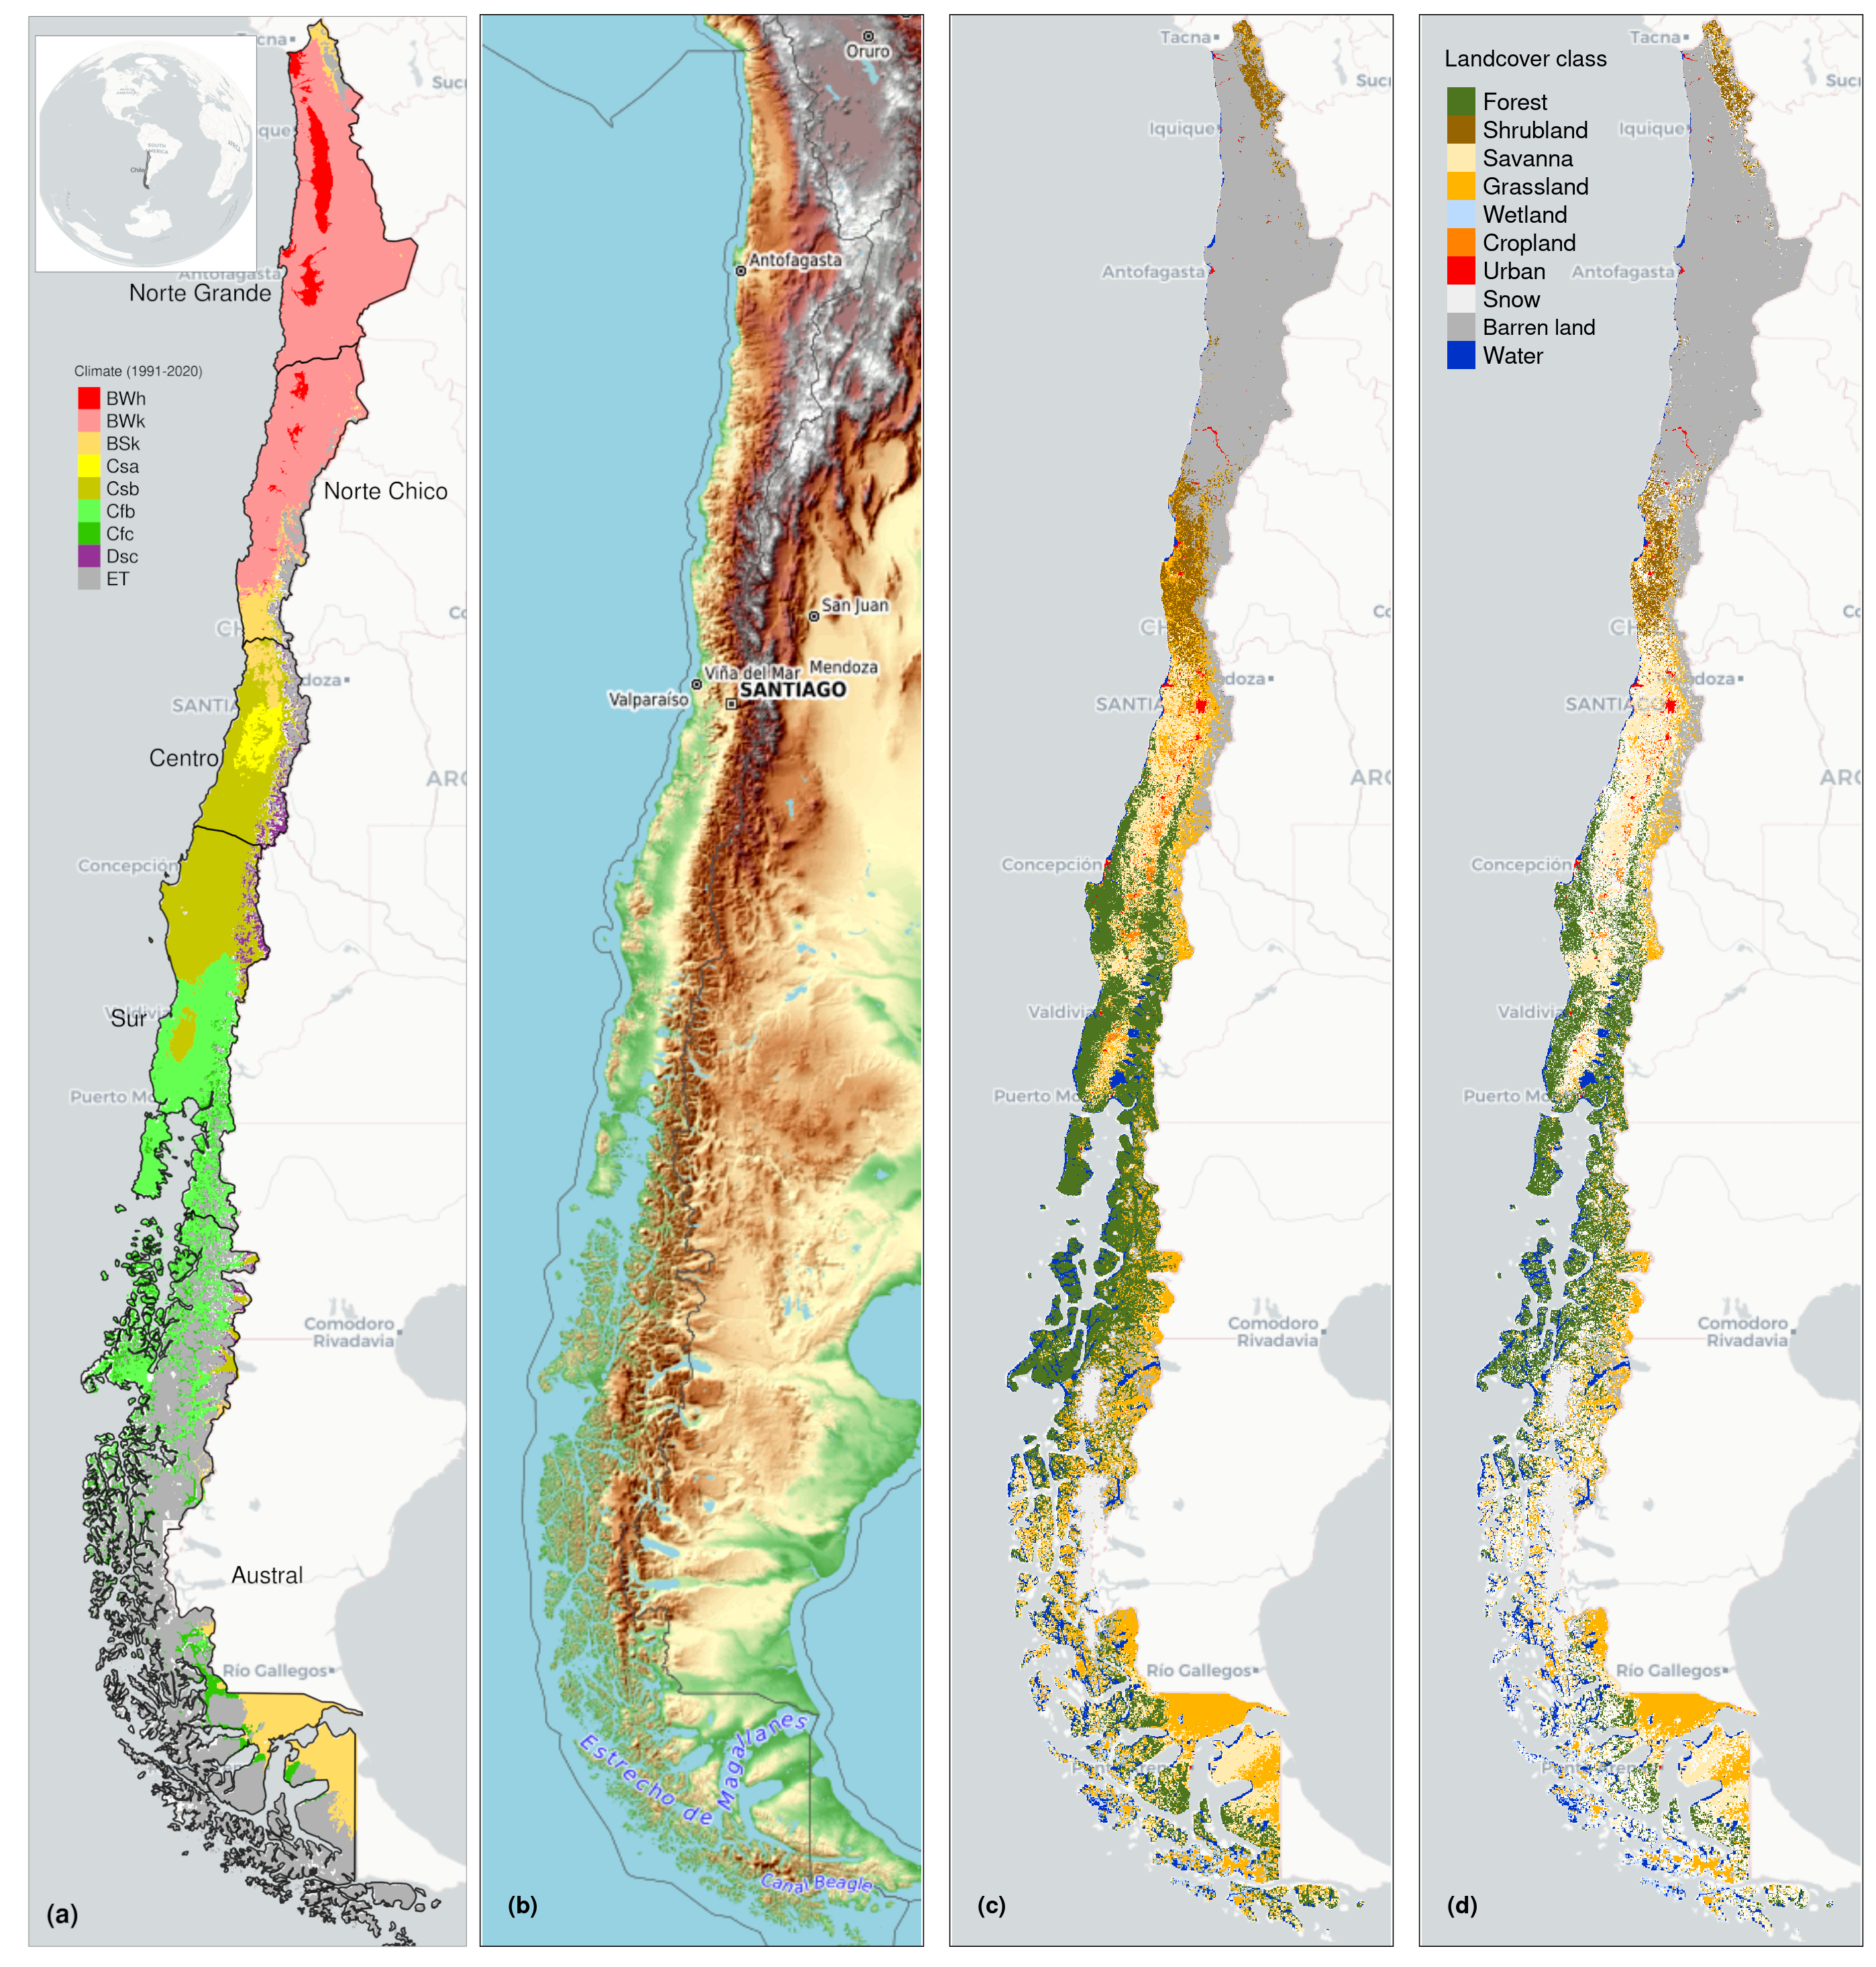
\includegraphics{figs/map_study_con_landcover.png}

}

\caption{\label{fig-studyArea}(a) Chile with the Koppen-Geiger climate
classes and the five macrozones ``Norte Grande'', ``Norte Chico'',
``Centro'', ``Sur'', and ``Austral''. (b) Topography reference map. (c)
land cover classes for 2022. (d) Persistent land cover classes
(\textgreater{} 80\%) for 2001-2022.}

\end{figure*}%

\subsection{Data}\label{data}

\subsubsection{Gridded meteorological and vegetation
data}\label{gridded-meteorological-and-vegetation-data}

To derive a proxy for vegetation productivity, we used the Normalized
Difference Vegetation Index (NDVI) from the product MOD13A3 Collection
6.1 from MODIS . MOD13A3 provides vegetation indices with a 1 km spatial
resolution and monthly frequency \citep{Didan2015}. For soil moisture,
water supply, and water demand variables, we used ERA5-Land (ERA5L)
(ECMWF Reanalysis version 5 over land) \citep{MunozSabater2021}, a
reanalysis dataset that provides atmospheric and land variables since
1950. It has a spatial resolution of 0.1° (9 km), hourly frequency, and
global coverage. We selected total precipitation, maximum and minimum
temperature at 2 meters, and volumetric soil water layers between 0 and
100 cm of depth (layer 1 to layer 3; Table SSX).

\subsection{Short- to long-term drought
trends}\label{short--to-long-term-drought-trends}

\subsubsection{Atmospheric Evaporative Demand
(AED)}\label{atmospheric-evaporative-demand-aed}

To compute drought indices that use water demand, it is necessary to
first calculate AED. To do this, we employed the Hargreaves method
\citep{Hargreaves1994, Hargreaves1985} by applying the following
equation:

\begin{equation}\phantomsection\label{eq-AED}{AED = 0.0023\cdot Ra\cdot (T+17.8)\cdot (T_{max}-T_{min})^{0.5}}\end{equation}

where \(Ra\) \((MJ\,m^2\, day^{-1})\) is extraterrestrial radiation;
\(T\), \(T_{max}\), and \(T_{min}\) are mean, maximum, and minimum
temperature \((°C)\) at 2m. For calculating \(Ra\) we used the
coordinate of the latitud of the centroid of each pixel as follow:

\begin{equation}\phantomsection\label{eq-Ra}{R_a = \frac{14,400}{\pi}\cdot G_{sc}\cdot d_r \left[\omega_s\cdot sin(\phi)\cdot sin(\delta)+cos(\phi)\cdot cos(\delta)\cdot sin(\omega_s) \right]}\end{equation}

where:

\(Ra\): extraterrestrial radiation \([MJ\, m^{-2} day-1]\),\\
\(G_{sc}\): solar constant = 0.0820 \([MJ\,m^{-2} min^{-1}]\),\\
\(d_r\): inverse relative distance Earth-Sun,\\
\(\omega_s\) sunset hour angle \([rad]\),\\
\(\phi\): latitude \([rad]\),\\
\(\delta\): solar declination \([rad]\).

We selected the method of Hargreaves to estimate AED because of its
simplicity, as it only requires temperature and extraterrestrial
radiation, and because access to the data needed for alternative methods
(e.g., Penman-Montieth) is often limited \citep{Vicente-Serrano2014}.

\subsubsection{Drought indices}\label{drought-indices}

To derive the drought indices of water supply and demand we used the
ERA5L dataset and the MODIS product (MOD13A3\citep{Didan2015b}), with a
monthly frequency for 1981--2023 and 2000--2023, respectively. Drought
indices capture historical anomalies of water supply and demand. To
quantify each anomaly, the common practice is to derive it following a
statistical parametric method in which it is assumed that the
statistical distribution of the data is known \citep{Heim2002}. The use
of an erroneous statistical distribution that does not fit the data is
usually the highest source of uncertainty \citep{Laimighofer2022}. In
the case of Chile, due to its high degree of climatic variability, it is
difficult to choose a statistical distribution that can be used across
its entire extent. We therefore use a non-parametric method for the
calculation of the drought indices, following \citet{Farahmand2015}.

For monitoring water supply, we used the Standardized Precipitation
Index (SPI; \citet{McKee1993}), which relies on precipitation data. To
evaluate water demand, we chose the Evaporative Demand Drought Index
(EDDI; \citet{Hobbins2016} and \citet{McEvoy2016}), which is based on
the AED. To consider the combined effect of water supply and demand, we
selected the SPEI \citep{Vicente-Serrano2010}. For SPEI, an auxiliary
variable \(D=P−AED\) is calculated. Soil moisture is the main driver of
vegetation productivity, particularly in semi-arid regions
\citep{Li2022}. Hence, we used the Standardized Soil Moisture Index
(SSI) to monitor soil moisture (SM) \citep{Hao2013}. For the SSI, we
used the average soil moisture from ERA5L at a depth of 1m. All
calculated indices are multi-scalar and can be used for the analysis of
short- to long-term droughts.

To derive the drought indices, we first calculate the sum of the
variables with regard to the time scale(s). In this case, for
generalization purposes, we will use \(V\), referring to variables P,
AED, D, and SM (Table SSX). We accumulated each over the time series of
values (months), and for the time scales s:

\begin{equation}\phantomsection\label{eq-sumvar}{A^s_i = \sum_{i=n-s-i+2}^{n-i+1} V_i\,\, \forall\, i\geq n-s+1  }\end{equation}

The \(A^s_i\) corresponds to a moving window (convolution) that sums the
variable for time scales \(s\). This is summed over \(s\) months,
starting from the most recent month (\(n\)) back in time until month
\(n-s+1\). For example, using as a variable the precipitation, a period
of twelve months (\(n\)), and a time scale of three months (\(s\)):

\[
\begin{split}
A^3_1 &= P_{oct} +P_{nov} +P_{dic} \\
\vdots\,\,\, &= \,\,\,\vdots + \,\,\,\vdots + \,\,\,\vdots \\
A^3_{10} &= P_{jan}+P_{feb} +P_{mar}
\end{split}
\]

Then, we used the empirical Tukey plotting position \citep{Wilks2011}
over \(A_i^s\) to derive the \(P(A_i^s)\) probabilities across a period
of interest:

\begin{equation}\phantomsection\label{eq-probPai}{P(A^s_i) = \frac{i-0.33}{n+0.33'}}\end{equation}

An inverse normal approximation \citep{Abramowitz1968} obtains the
empirically derived probabilities once the variable cumulates over time
for the scale \(s\). Thus, the drought indices \(SPI\), \(SPEI\),
\(EDDI\), and \(SSI\) are obtained following the equation:

\begin{equation}\phantomsection\label{eq-DI}{DI(A^s_i) = W - \frac{C_0+C_1\cdot W + c_2 \cdot W^2}{1+d_1\cdot W +d_2\cdot W^2 +d_3\cdot W^3}}\end{equation}

\(DI\) is referring to the drought index calculated for the variable
\(V\). The values for the constats are: \(C_0 = 2.515517\),
\(C_1 = 0.802853\), \(C_2 = 0.010328\), \(d_1 = 1.432788\),
\(d_2 = 0.189269\), and \(d3 = 0.001308\). For \(P(A^s_i) \leq 0.5\),
W=\(\sqrt{-2\cdot ln(P(A^s_i))}\) , and for \(P(A^s_i) > 0.5\), replace
\(P(A^s_i)\) with \(1-P(A^s_i)\) and reverse the sign of \(DI(A^s_i)\).

The drought indices were calculated for time scales of 1, 3, 6, 12, 24,
and 36 months at a monthly frequency for 1981--2023.

\subsubsection{Temporal trends of drought
indices}\label{temporal-trends-of-drought-indices}

To determine if there are statistically significant positive or negative
temporal trends for the drought indices, we used the non-parametric
modified Mann-Kendall test for serially correlated data \citep{Yue2004}.
To determine the magnitude of the trend, we used Sen's slope
\citep{Sen1968}. Sen's slope is less affected by outliers than
parametric ordinary least squares regression, and as a non-parametric
method it is not influenced by the distribution of the data. We applied
both methods for SPI, EDDI, SPEI, and SSI and six time scales, resulting
in a total of 24 trends. We then aggregated temporal trends for each
region and land cover type.

\subsection{Vegetation productivity}\label{vegetation-productivity}

We also used the MODIS product to calculate vegetation productivity, and
calculated anomalies in NDVI using zcNDVI \citep{Zambrano2018}, which
was derived from the monthly time series of NDVI, with Equations
Equation~\ref{eq-sumvar} and Equation~\ref{eq-DI}. For vegetation
productivity, we selected the time scale that best correlates with
annual net primary productivity (NPP) across continental Chile. For this
purpose, we calculated zcNDVI for time scales of 1, 3, 6, and 12 months
(from December) and compared it with the annual NPP. We obtained NPP
from MOD17A3HGF \citep{Running2019}. We chose to use six months because
the \(R^2\) between zcNDVI and NPP reaches its highest value at six
months, obtaining an \(R^2\) of 0.31 for forest and 0.72 for shrubland
(Supplementary Information Section S5). We subsequently used zcNDVI with
a time scale of 6 months and calculated it at a monthly frequency for
2000--2023.

\subsubsection{Drought impacts on vegetation
productivity}\label{drought-impacts-on-vegetation-productivity}

For each land cover, we analyzed the trend of vegetation productivity.
To this end, we identified areas within each land cover macro-class that
are persistent over time, to reduce the possibility that trends in
vegetation productivity may be influenced by changes in land cover. We
examined the correlation between drought indices and vegetation
productivity across land cover types to determine to the extent to which
soil moisture and water demand and supply affect vegetation
productivity.

We estimated pixel-to-pixel Pearson's correlations between drought
indices at time scales of 1, 3, 6, 12, 24, and 36 months with zcNDVI. We
extracted the Pearson correlation coefficient corresponding to the time
scale with the highest value. For each index, we then generated two
raster maps: 1) a raster with values of the time scales and drought
index that reached the maximum correlation, and 2) a raster with the
magnitude of the correlation between the drought index and vegetation
productivity.

\subsection{Drought impacts on land cover
change}\label{drought-impacts-on-land-cover-change}

\subsubsection{Land cover change}\label{land-cover-change}

To analyze land cover change, we used the classification scheme of the
International Geosphere-Biosphere Programme (IGBP) from the product
MCD12Q1 Collection 6.1 from MODIS. The MCD12Q1 product is produced for
each year from 2001 to 2022 and defines 17 classes (see Table Sx).
Following the FAO classification \citep{FAO2022}, we considered native
and planted forests as ``forests'', which represent natural and
productive ecosystems dominated by large trees. To analyze the land
cover change, we use the IGBP scheme from the MCD12Q1 Collection 6.1
from MODIS. We regrouped the 17 classes into ten macro-classes, as
follows: 1-4 to forests (native forest and plantations), 5-7 to
shrublands, 8-9 to savannas, 10 as grasslands, 11 as wetlands, 12 and 14
to croplands, 13 as urban, 15 as snow and ice, 16 as barren, and 17 as
water (Table S1). This resulted in a time series of land cover with ten
macro-classes for 2001 and 2023. We validated the land cover
macro-classes using a high resolution (30m ) land cover map for
2013-2014 \citep{Zhao2016}. Our results showed a global accuracy of
\textasciitilde0.82 and a F1 score of \textasciitilde0.66 (Supplementary
Information, S2).

We calculated the area for each land cover class in the five study
regions for 2001--2022. We then estimated the temporal change in area
for each land cover type and macro-class, and determined the statistical
significance and magnitude of the trend as described above. To assess
how water demand and supply, and soil moisture affect the variation in
vegetation productivity across various land cover types, we avoid
analyzing areas that experienced major land cover changes in the
2001--2022 period. To assess how zcNDVI varied irrespective of land
cover change, we developed a persistence mask for land cover, which only
retains pixels for which the macro-class remained the same for at least
80\% of the 22 years (Figure~\ref{fig-studyArea} d).

\subsubsection{Relationship between land cover and drought
trends}\label{relationship-between-land-cover-and-drought-trends}

To identify which drought indices and time scales have a major impact on
changes in land cover type, we examined the relationship between the
trend in land cover classes and the trend in drought indices. We
performed the analysis at the sub-basin scale, using 469 basins, which
have a surface area between 0.0746 and 24,000 \(km^2\) and a median area
of 1,249 \(km^2\). For each basin, we calculated the trend per land
cover type, considering the proportion of the type relative to the total
surface of the basin. For each basin we extracted the average trend of
all drought indices and at time scales of 1, 3, 6, 12, 24, and 36
months. Also, we extracted the average trend in zcNDVI.

We modeled trends in land cover type per macroclass with the aim of
assessing how land cover trends relate to drought indices. We used the
random forest method \citep{Ho1995}, which employs multiple decision
trees, allowing for classification and regression. Some advantages
include the ability to find non-linear relationships, reduce
overfitting, and derive variable importance. We included the four
drought indices at each time scale and zcNDVI for a total of 25
predictors and built six random forest models, one for each land cover
and region. We trained each model with 1000 trees using a resampling
strategy with cross-validation. To this end, we used cross-validation to
evaluate model fit using ten folds then calculated \(R^2\), root mean
square error (RMSE), and variable importance. Variable importance
identifies which variables have a higher contribution to explaining
model variation. We calculated variable importance by permuting
out-of-bag (OOB) data per tree and calculating the mean standard error
of the OOB data. After permuting each predictor variable, we repeated
the process for the remaining variables. We repeated this process ten
times per fold to assess model fit. Finally, we visually explored the
relationship between drought indices and changes in land cover. To do
this, we compared the relative changes in land cover surface with the
drought indices of six and thirty-six months.

\subsection{Software}\label{software}

For the downloading, processing, and analysis of the spatio-temporal
data, we used the open source software for statistical computing and
graphics, R \citep{R2023}. For downloading ERA5L, we used the \{ecmwfr\}
package \citep{Hufkens2019}. For processing raster data, we used
\{terra\} \citep{Hijmans2023} and \{stars\} \citep{Pebesma2023}. For
managing vectorial data, we used \{sf\} \citep{Pebesma2018}. For the
calculation of AED, we used \{SPEI\} \citep{Bergueria2023}. For mapping,
we used \{tmap\} \citep{Tennekes2018}. For data analysis and
visualization, the suite \{tidyverse\} \citep{Wickham2019} was used. For
the random forest modeling, we used the \{tidymodels\} \citep{Kuhn2020}
and \{ranger\} \citep{Wright2017} packages.

\section*{Acknowledgments}\label{acknowledgments}
\addcontentsline{toc}{section}{Acknowledgments}

The National Research and Development Agency of Chile (ANID) funded this
study through the drought emergency project FSEQ210022, Fondecyt
Iniciación N°11190360, Fondecyt Postdoctorado N°3230678, and Fondecyt
Regular N°1210526.

\section{References}\label{references}

\renewcommand{\bibsection}{}
\bibliography{references.bib}




\end{document}
